\documentclass[11pt,letterpaper]{article}
\usepackage{graphicx}
%\usepackage{cite}
\usepackage{url}
\usepackage{amsmath}
\usepackage{amssymb}
\usepackage{color}
\usepackage{wrapfig}
\usepackage[sort&compress]{natbib}
\usepackage[bookmarks=false,colorlinks,citecolor=blue,urlcolor=blue]{hyperref}

\include{basic-macros}

\setlength{\textheight}{9in}
\setlength{\topmargin}{0in}
\setlength{\headheight}{0in}
\setlength{\headsep}{0in}
\setlength{\textwidth}{6.5in}
\setlength{\oddsidemargin}{0in}

\newcommand{\equationsize}{\small}
\newcommand{\bibliographysize}{\small}
\newcommand{\captionsize}{\small}
\newcommand{\captionspace}{\vspace*{-0.2in}}
\newcommand{\afterfigspace}{\vspace*{-0.2in}}

\newcommand{\Section}[1]{\vspace*{-0.08in}\section{#1}\vspace*{-0.08in}}
\newcommand{\SubSection}[1]{\vspace*{-0.08in}\subsection{#1}\vspace*{-0.08in}}
\newcommand{\SubSubSection}[1]{\vspace*{-0.08in}\subsubsection{#1}\vspace*{-0.08in}}

% set spacing in figure caption
\newcommand{\figurespacing}{\renewcommand{\baselinestretch}{1.0}}

% symbol footnote: use \symbolfootnote[#]{footnote} to invoke with
%    1 = *; 2 = dagger; 3 = double-dagger; 4--9 = see latex docs
\long\def\symbolfootnote[#1]#2{\begingroup%
\def\thefootnote{\fnsymbol{footnote}}\footnote[#1]{#2}\endgroup}

% bold paragraph headers
\newcommand{\boldstart}[1]{\vspace{0.07in}\noindent{\bf #1}}

\newcommand{\comment}[1]{}
\newcommand{\todo}[1]{{\textcolor{red}{\bf [#1]}}}
\newcommand{\todd}[1]{{\color{red}{[\emph{TZ: #1]}}}}

% math shortcuts -- from Todd
\newcommand{\vx}{{\bf x}}
\newcommand{\vy}{{\bf y}}


% math shortcuts -- from Trevor
\newcommand{\rep}{{\bf f}}
\newcommand{\repc}{{f}}
\newcommand{\repg}{{\bf g}}
\newcommand{\repgc}{{g}}
\newfont{\msym}{msbm10}
\newcommand{\reals}{\mbox{\msym R}}
\newcommand{\params}{{\bf w}}
\newcommand{\proj}{{\bf A}}
\newcommand{\allparams}{{\bf W}}
\newcommand{\paramsv}{{\bf v}}
\newcommand{\paramsu}{{\bf u}}
\newcommand{\auxi}{{\cal T}_i}

% Euclidian space R^{n}. Needs \usepackage{amssymb}
\newcommand{\Rn}[1]{{\mathbf  R}^{#1}}

\graphicspath{{figs/}}

\def\mytitle{{{\small CIF: Small:}\vspace{0.05in}\\ {\Large Foundations for Social Image Analytics: From Images to Social Graph}}}

\begin{document}

%%% THIS PAGE UPLOADED AS SUPPLEMENTARY DOCUMENTS %%%
%\pagestyle{empty}
%\begin{enumerate}
%\item Todd Zickler; Harvard University; PI
%\item Todd Zickler; Harvard University; co-PI
% \end{enumerate}

%%% THIS PAGE UPLOADED AS PROJECT SUMMARY %%%
\pagebreak

% !TEX root = SocialVision2012.tex
\pagestyle{empty}

\noindent\textsf{CIF: Small:}\vspace{0.9ex}\\
\noindent {\bf \textsf{\Large Foundations for Social Image Analytics: From Images to Social Graph}}

\vspace{1.0ex}
\noindent \textsf{\large \em Todd Zickler and Ruonan Li, Harvard University}
\vspace{2.0ex}



\noindent Large-scale image/video collections contain rich information about human interactions, relationships, and social structure: Whether it is a personal collection, a shared collection of an online community, or a collection from a surveillance network, any large set of visual observations of people over an extended period of time provides access to co-occurrence counts, relative face and body positions, gestures, expressions, as well as scene and event types, all of which provide information about identities, attributes, interactions, and relationships, which is richer and more nuanced than that from textual signals like email logs, phone logs, and textual social media. This proposal aims to develop a computational foundation for image/video processing systems that can recognize social interactions and extract social relationship and social network from image/video collections. 

These systems will extract, from images/videos of human gatherings, information about the types and frequencies of social interactions that occur, and information about the social network, represented as a social graph, which embeds the observed individuals. This information will undoubtedly be useful for machines, just as it is useful for humans when analyzing individuals within a social group from a distance; when deciding which colleagues to approach to enact policy changes; or when judging whether to alert authorities of a questionable interaction between strangers: If we had good tools for analyzing relationships and social networks from images, we could build better tools for discovering interaction patterns and inter-personal structures in active classrooms, sports matches, and other public spaces, and we could also build better human-computer interfaces, recommendation systems, video indexing methods, and security systems.

\boldstart{Intellectual Merit}. Achieving our goals requires coordinated innovation in two areas: semantic image processing for distill social interactions, and multidimensional signal processing on graphs for establishing the social network.  For the former, we will introduce representations of interactions and relational attributes based on proxemes---the interaction-analogy to phonemes in speech---that are modulated by the social roles and relationship between the actors. We will introduce models and similarity measures for proxemes that provide a foundation for the learning of proxeme vocabularies from annotated data, and the detection of proxeme occurrences in images and videos. In concert with these innovations, we will use spatio-temporal distributions of proxemes to define new functionals on social graphs (cell complexes) and develop tools to extremize these functionals. As a concrete example, one such extremization would simultaneously produce: 1) the number of unique individuals (0-cells, or nodes); 2) the identification of actors in each scene with their corresponding 0-cells; 3) personal attributes at each 0-cell, such as age and gender; 4) multi-dimensional signals of relational attributes at the 1-cells (edges), such as parent-child, friends, or colleagues; and 5) communal attributes at higher-order cells.

\boldstart{Broader Impacts}. The proposed research will provide a foundation for socially-aware image processing systems that have the potential to transform security, surveillance, augmented reality, human computer interaction, human resource planning, operations research, and e-commerce. It will also benefit computational research in sociology, economics, and education by providing researchers with access to social patterns that are difficult or impossible to detect with the naked eye. The results of this research will be broadly disseminated by making datasets and software publicly available and by producing publications in refereed conferences and journals. The program will also impact education at the undergraduate and graduate levels, including giving undergraduates the opportunity to gain hands-on research experiences in participating in the research activity. 

\boldstart{Keywords:} Semantic Image processing; Social Network; Multi-dimensional Signals on Graphs

\comment{Three challenges combine to make this problem distinctive: 1) behaviors and interaction types must be inferred from imagery and are therefore noisy and ambiguous; 2) in addition, there is ambiguity in who is interacting because actor identities must also be inferred; and 3) like other network-inference problems, community structures exist at multiple scales, and measurements are incomplete because of unobserved co-occurrences. Meeting these challenges}  

%%%%%%%%% 2014 version %%%%%%%%%%%%%%%%


%\noindent This proposal aims to develop a computational foundation for computer vision systems that are socially-aware, in the sense of being able to recover from imagery information about social relationships and social networks. These systems will extract, from collections of images and videos of human gatherings, information about the types and frequencies of social interactions that occur, as well as information about the social network that embeds the observed individuals. This information will undoubtedly be useful for machines, just as it is useful for humans when analyzing individuals within a social group from a distance; when deciding which colleagues to approach to enact policy changes; or when judging whether to alert authorities of a questionable interaction between strangers.
%
%
%The proposed research will introduce computer vision as a new source of social network information, one that complements email logs, phone logs, web-based community connections, and so on. Vision is an important complement to these because it provides access to face positions, body poses, gestures, expressions, and scene types, all of which are difficult to observe by any other means but are critical signals for analyzing interactions and relationships.
%
%
%This research is timely because of the recent maturation of technologies for detecting and tracking the faces and bodies of people and recognizing their identities. A variety of practical systems exist, and by integrating them one can extract crude but useful descriptors of individual behaviors in the form of positions, trajectories, body poses, and so on. When image quality permits, these can also be augmented with more detailed per-individual descriptors computed from gestures  and facial expressions. In any case, with these descriptors an image (resp. video) can be abstracted as a collection of noisy per-agent detections (resp. trajectories) with accompanying (uncertain) behavior descriptors, and this is the abstraction on which the proposed framework will operate.

%\boldstart{Intellectual Merit}. Extracting social relationships and social networks from imagery poses several technical challenges, including: 1) representing interactions, and learning ``proxemes" --- interaction categories that are informative about relationships --- in semi-supervised and unsupervised settings; 2) detecting and recognizing proxemes in images or videos of large social gatherings; 3) inferring mixed-membership social networks from proxemes, accounting for noisy inputs and uncertain identities; and 4) collecting and disseminating meaningful datasets for development and evaluation. To address these challenges, the PIs will draw upon their expertise in analyzing individual and group behaviors; recognizing identities from faces embedded in a social network; creating public benchmark datasets; and enabling efficient learning by adapting recognition systems between different domains.






%%%%%%%%%%%%%%%%%%%%%%%%%%%%%%%%%

%\noindent This proposal aims to develop a computational foundation for computer vision systems that are socially-aware, in the sense of being able to recover from imagery information about social interactions and social relationships. These systems will extract, from collections of images and videos of human gatherings, information about the types and frequencies of social interactions that occur, as well as information about the social network that embeds the observed individuals. This information will undoubtedly be useful for machines, just as it is useful for humans when analyzing individuals within a social group from a distance; when deciding which colleagues to approach to enact policy changes; or when judging whether to alert authorities of a questionable interaction between strangers.


%We propose a framework to \emph{see} a social network - one that exploits images and videos and employs computer vision as a new `sensor' by which we aim to recover social relationships and attributes among individuals in our social communities. Contemporary research on social networks has been revealing us rich semantics by exploiting diverse `conventional social sensors' from textual/voice communications to online message sharing, but it has almost completely ignored visual media from abundant online photos to video volumes harvested by surveillance camera networks. Camera, as a new `community sensor', is much less intrusive than conventional social sensors, but exposes us the `real stories' about the community members from aside and remotely: Many of these stories may be too subtle for conventional approaches to grasp but visually sensible. Cameras, equipped with ever-increasing computer vision capabilities, produce socially-informaive data in a quantity thousand times of what conventional sensors do, but these data has largely remained unexplored for social networks. It is now our mission to introduce vision to social networks in this proposed research agenda.
%
%In companion, we propose to understand images and videos by incorporating the contextual knowledge provided by the online social connections where the images and videos are embedded, as well as to distill from images and videos new social semantics previously only under the attention of conventional sociology. This effort builds upon, but will go much beyond the preliminary attempt on recognizing faces and identities under social contexts: Face recognition only tells about \emph{who} are in the visual scene, but we argue that benefits from the socialized nature of media nowadays are not limited to the task of `who'. Knowing more about the social connections among the visual documents helps us to better understand \emph{what} the individuals are doing therein and \emph{where} they geographically are, and even enables us to predict more precisely \emph{whether} a particular event is to happen next.
%
%In fact, both the visual sensing of a social network and the socially assisted understanding of visual materials can benefit from cross-pollination: Visually sensed social ties provide more specific contextual evidences about who are more likely to interact in a new visual scene and what activities they are more likely to be engaged in, while watching the visual co-occurrences and co-activities of two community members may reflect more accurate connections between them that are not easily available from other resources. By socially-aware visual analytics, we mean a comprehensive theoretical and practical infrastructure that we expect to develop during the award period, with the two complementing modules of the visual sensing of a network and the socially assisted visual understanding well integrated.
%
%\boldstart{Intellectual Merit}. We propose a paradigm for socially-aware visual analytics, which systematically explores the interactions between visual information and social communities, yielding a new foundation for machine discovery of sociological knowledge and the potential for new perspectives and applications in visual understanding and computer vision. The paradigm includes new models and representations for networks arising from exploiting visual concepts in images and videos, and includes computational mechanisms to leverage socialized metadata for the new tasks in image and video analysis. The paradigm will, in particular, account for realistic situations in network sensing, such as multi-type overlapping communities and partial noisy observations, which has been largely overlooked by contemporary research, and all novel functionalities will build on mature elements in computer vision, such as face/human detection, recognition, and tracking, scene analysis, and event/activity interpretation, and will be deployed in the form of software and hardware.

%\boldstart{Intellectual Merit}. Extracting social interactions and social relationships from imagery poses several technical challenges, including: 1) learning models for social interaction categories, including in semi-superivsed and unsupervised settings; 2) detecting and recognizing interaction categories in long videos of large social gatherings; 3) inferring mixed-membership social networks from multiple noisy visual sources and uncertain identities; and 4) collecting and disseminating meaningful datasets for development and evaluation. To address these challenges, the PIs will draw upon their expertise in analyzing individual and group behaviors in videos; recognizing identities from faces embedded in a social network; creating public benchmark datasets; and enabling efficient learning by adapting recognition systems between different domains.

%
%\boldstart{Broader Impacts}. The primary application domain of the proposed research is online and networked visual media about humans, while it will be also applicable to broader visual materials involving other agents, such as historical image archives, scientific image collections, biological recordings, and so on. Socialized behaviors are prevalent in social creatures, and our research will shed lights on new approaches to automatic browse, index, and parse them. New insights will be drawn toward diverse disciplines spanning sociology, pedagogy, and statistics, which are still in their infancy in introducing automated approaches exploiting visual information. Besides the tremendous potentials of industrial interests and product implementation that do not need elaboration, the proposed interdisciplinary research will also prompt revolutions in educational programs providing next-generation students with more comprehensive knowledge and broader mastery of skills.


\pagebreak

% !TEX root = SocialVision2014.tex
\pagestyle{plain} \pagenumbering{arabic}

\Section{Introduction} \label{sec:intro}

Image and video collections contain rich information about human interactions, human relationships, and social structure. Whether it is a personal collection, a shared collection of an online community, or a collection from a surveillance network, any large set of visual observations of people over an extended period of time provides access to co-occurrence counts, relative face and body positions, gestures, expressions, and scene types, all of which provide information about identities, attributes, interactions, and relationships. This social information is richer and more nuanced than that from textual signals like email logs, phone logs, and textual social media, and it will undoubtedly be useful for machines, just as it is useful for humans when analyzing individuals within a social group from a distance; when deciding which colleagues to approach to enact policy changes; or when judging whether to alert authorities of a questionable interaction between strangers. If we had good tools for analyzing behaviors and relationships in large image and video collections, we could build better tools for discovering interaction patterns and social structures in active classrooms, sports matches, and  public spaces. We could also build better human-computer interfaces, recommendation systems, video indexing methods, and security systems.
 
This project will develop a foundation for these applications by an introducing image and signal processing paradigm for recognizing interactions and extracting social information from large-scale imagery. We will develop tools to extract, from images and videos of human gatherings,  information about the types and frequencies of social interactions that occur, as well as compute useful information about the underlying social network, represented as a social graph that embeds the individuals, groups, and communities, and that describes their relationships.  This research will introduce images and video as a new source for ``sensing" social networks and estimating signals on social graphs. This will complement emails, phone logs, and web-based media by exploiting face positions, body poses, movements, and scene and event types --- things that are critical for analyzing interactions and relationships, but are difficult to observe by any means other than images.


We will achieve our goals by coordinated innovations in two areas: \emph{semantic image processing} and \emph{multidimensional signal processing on (social) graphs}, as shown in Figure~\ref{fig:intro}. For the former, we will exploit the fact that social interactions between two or more people can be broken down into basic spatial and spatio-temporal visual elements; that these visual elements can be usefully categorized; and that the frequency and structure of occurrences of these elemental categories carry information about actors' roles and relationships. These ideas are rooted deeply in anthropological and sociological studies of non-verbal communication, and in this proposal, we borrow and broaden the anthropological term \emph{proxemes} to refer to the basic elements of social interactions. For us, a proxeme can be a relative spatial arrangement of two or more people at a particular instance of time (static; observable in an image), or a space-time sequence of such arrangements (dynamic; observable in a video), and proxemes can exist at many different spatial and temporal resolutions. We will develop semantic image processing tools that detect, recognize, and summarize the spatio-temporal occurrences of the proxemes in image and video collections, based on visual features---from coarse bag-of-words features to explicit, fine-scale pose estimates---that are appropriate for the quality and resolution of the input data.

For our second area of innovation, multidimensional signal processing on graphs, we will develop a foundation for robustly translating the noisy relationship information implied by detected visual proxemes into an estimate of the social network that embeds the observed individuals. A social network is a graph (cell complex) whose nodes (0-cells) correspond to the observed individuals. Our goal is to infer for every edge (1-cell) the type of social relationship from among a dictionary of possibilities (parent-child, friends, partners, etc.). This suggests a representation where a $K$-vector is associated with each 1-cell, and where the $k$th element of the vector encodes the strength and direction of the pairwise link according to the $k$th relationship type. Relationship types are not independent in general (if A is a parent of B and C, then B cannot also be a parent of C), so we need to create new models and methods for analyzing multi-dimensional, or vector-valued, signals on edges. In particular, several challenges combine to make this problem distinctive: 1) proxemes must be inferred from imagery and therefore provide link information that is very noisy and ambiguous (although plentiful); 2) in addition to ambiguity in \emph{how} two targets are related socially, there is ambiguity in \emph{who} the targets are, because actor identities must also be inferred; and 3) like other network-inference problems, community structures exist at multiple scales and among higher-order cells, and measurements are incomplete because of unobserved co-occurrences.

\begin{figure}[t!]
\begin{center}
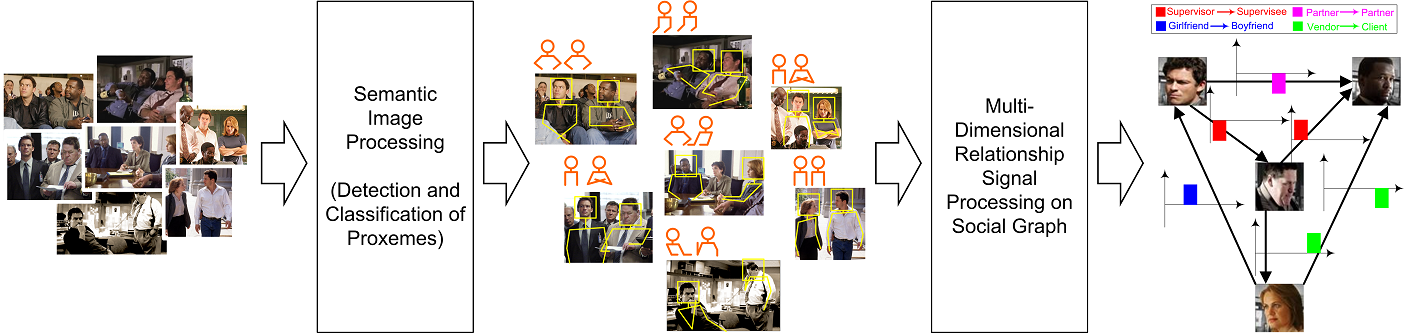
\includegraphics[width=\columnwidth]{overview}
\end{center}
\vspace{-0.25in} \caption{\captionsize 
Social visual analytics: A computational foundation for recovering social relationships and social networks from image and video collections. We will pursue two coordinated research directions: semantic image processing with a focus on detecting and classifying proxemes (elemental interactions), and multi-dimensional signal processing on social graphs. These two directions are summarized in Figures~\ref{fig:proxeme_det_recog} and~\ref{fig:SP_on_Graph} respectively. (Best viewed in color.)\label{fig:intro}\afterfigspace}
\end{figure}

The signal processing knowledge and tools required to solve these problems do not yet exist. We will create them by pursuing four related aims:

\begin{enumerate}

\vspace{-0.1in}\item \emph{Representing, detecting, and recognizing social proxemes.} We will develop efficient computational representations for elemental interactions (proxemes) based on mixed ensembles of per-actor descriptors and relative, between-actor descriptors. Along with these, we will co-develop processes for measuring the similarity between two interaction elements, thereby enabling learning of proxeme vocabularies from annotated data, as well as the detection and recognition of proxeme occurrences in large image and video collections of human gatherings. The detected and recognized proxemes, combined with other individual attributes such as gender, age, and social role, will provide ``observed'' noisy relationship signals.

\vspace{-0.1in}\item \emph{Robust graph coarsening.} To estimate a social graph, we must first identify the nodes in the graph. For every pair of detected actors/targets in an image set, one can compute a visual similarity score indicating the likelihood for the pair to belong to a single individual, and we will develop graph coarsening methods for reducing massive similarity graphs defined on all image targets to smaller graphs that contain the unique social members. We seek methods that robustly account for false face detections and non-participating ``by-standers'', and that are able to incorporate contextual constraints between targets, such as that an individual cannot co-occur with herself in the same image. 
%\comment{A similar scenario exists when determining a useful small dictionary of proxemes modulated by social relationships from a large set of interaction specimens, when proxemes are not directly defined by domain experts from social science, and therefore again requires robust graph coarsening framework. } 

%\vspace{-0.1in}\item \emph{Learning proxeme dictionaries.} Visual cues for human interactions at a cocktail party are very different from those in a boardroom meeting, which in turn are very different from those in a flipped classroom. Through decades of qualitative analysis, social scientists have catalogued some of the visual interaction elements in some of these settings; but due to the scarcity of qualified experts and the phenomenal manual effort this analysis requires, many visual elements have yet to be discovered. To address this, we will develop computational tools for supervised and semi-supervised learning of proxeme dictionaries. Our motivation is to use these dictionaries as intermediate representations for inferring social relationships, but they will also likely be useful for analyzing sports games, animal and cell populations, and many other situations that involve multiple interacting agents.

\vspace{-0.1in}\item \emph{Multi-dimensional signal processing on graphs.} Given identity and multi-dimensional relationship information from detected proxemes, we will develop filtering techniques for recovering clean multi-dimensional relationship signals on edges of a social graph. These techniques will respect semantic constraints between different relationship types (different dimensions). This requires new formulations that are distinct from existing analyses of signals on graph nodes, and we will create them by drawing on tools from graph theory and discrete calculus.

%\vspace{-0.1in}\item \emph{Inferring social networks from proxemes and other visual cues.} We will create computational methods for estimating social networks from multiple visual cues, including repeated occurrences of proxemes. Since existing network reconstruction tools are not optimized for visual input, we propose a suite of new techniques to improve performance when: (a) visual descriptors are derived from diverse, unreliable sources and are often missing, so proxeme counts are noisy; (b) the underlying social network contains multiple overlapping communities; and (c) the identities associated with detected and tracked agents are uncertain. 

\vspace{-0.1in}\item \emph{Data collection and challenge problems.} We will create datasets to evaluate our methods and design challenge problems to engage our colleagues in this research agenda. To do this, we will address the challenge of enabling reproducible research while preserving privacy.

\end{enumerate}

\vspace{-5pt}
The proposed research will provide a foundation for socially-aware signal/image systems that will transform national security, surveillance, human resource management, operations management, augmented reality, and human computer interfaces. The research will be carried out by a team with established expertise in semantic image processing for the recognition of identities, activities, and interactions, as well as the collection and analysis of social image and video collections. PI Todd Zickler has pioneered research on the use of social network context to improve image recognition~\cite{Stone2008,Stone2010} and led the implementation of a camera-based system for long-term observation of social interactions (Section~\ref{sec:sys}). PI Ruonan Li is an expert in video-based behavior analysis and activity recognition~\cite{groupdet2013,LiIJCV2012,LiPAMI2012,Li2010} and in adapting models when annotated training data is limited or difficult to obtain~\cite{LiZickler2012,Li2011}. 







%%%%%%%%%%%%%%%%%%%%%%% 2014 version %%%%%%%%%%%%%%%%%%%%%%%






%The past decade has produced stunning advances in computer vision. Real-time face detection introduced at the turn of the millennium is now commonplace in personal electronics. Face recognition has evolved from a research topic to a widely-used tool for managing photo albums. Systems such as Microsoft Photosynth and Google Earth can automatically reconstruct massive 3D models, and our ability to distinguish between object categories has improved dramatically, enabling applications from image search to product identification. If the mission of computer vision is to extract from imagery useful information about the world, it is clear that we now have functioning systems for more than a few types of information. 

%Yet, there are aspects of the world to which computer vision remains quite blind. Prominent among these are social interactions and social relationships between people. This information would undoubtedly be useful for machines, just as it is useful for humans when analyzing individuals within a social group from a distance; when deciding which colleagues to approach to enact policy changes; or when judging whether to alert authorities of a questionable interaction between strangers.

%We propose to develop foundations for computer vision systems that are `socially aware', in the sense of being able to recover social information from imagery. These systems will extract, from images and videos of human gatherings,  information about the types and frequencies of social interactions that occur; and they will  compute useful information about the social network that embeds the individuals, groups, and communities.  Our work will introduce computer vision as a new source of social network information, one that complements emails, phone logs, web-based community connections, and so on. Vision is an important complement to these because it provides access to face positions, body poses, movements, and scene types, all of which are difficult to observe by any other means but are critical for analyzing interactions and relationships. 

%We will achieve our goals by exploiting the fact that social interactions between two or more people can be broken down into basic spatial and spatio-temporal visual elements; that these visual elements can be usefully categorized; and that the frequency and structure of occurrences of these elemental categories carry information about interpersonal communications and relationships. These ideas are  rooted deeply in  anthropological and sociological studies of non-verbal communication, and in this proposal, we borrow and broaden the anthropological term \emph{proxemes} to refer to the basic elements of social interactions. For us, a proxeme can be a relative spatial arrangement of two or more people at a particular instance of time (static; observable in a photograph), or a space-time sequence of such arrangements (dynamic; observable in a video). With this definition in hand, our project can be described in four parts:




%\begin{figure}[t!]
%\begin{center}
%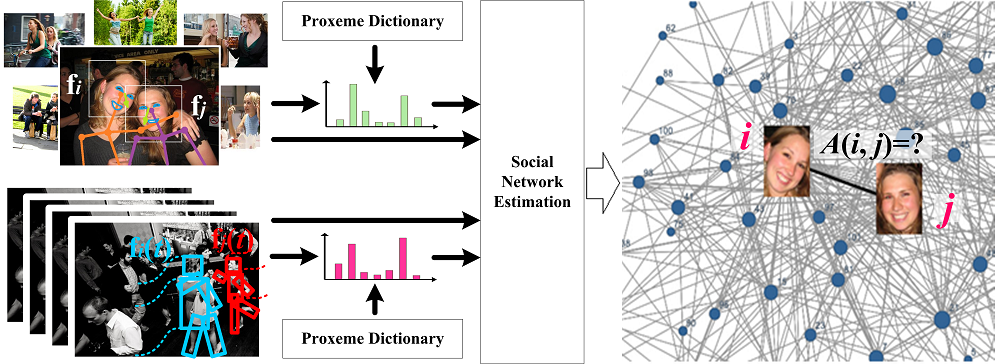
\includegraphics[width=\columnwidth]{intro_2014}
%\end{center}
%\vspace{-0.25in} \caption{\captionsize 
%Social visual analytics: A computational foundation for recovering information from image and video collections about social relationships and social networks through social proxemes. \label{fig:intro}\afterfigspace}
%\end{figure}
%





\comment{related work:
Study of non-verbal communication. Hall describes a set of four categories of inter-personal distances, and later equates the term `proxeme' with the phoneme of language~\cite{Hall}. Birdwhistell defines `kineme' as the minimal unit of an individual's visual expression (body movement, facial expression, or gesture). Kendon talks about interaction units that are space-time structures of \emph{relative} visual expressions, and introduces categories known as `f-formations' (see Fig.~X). We use the phrase proxeme.

"kineme" is "similar to a phoneme because it consists of a group of movements which are not identical, but which may be used interchangeably without affecting social meaning". (Knapp 1972:94-95)

, including areas of proxemics~\cite{hall} and kinesics~\cite{birstwell}. Kendon formalizes this procedure in video as context analysis, can be seen a particular instance of the analytical process of \emph{coding} used for qualitative analysis in social science. In this process, a set of categories are \emph{codes} are produced by experts through repeated observations of videos. rough definition of codes. We seek to automate this process.

Inspired by computational sociology~\cite{hall1974,Kendon1990,Lazer2009,Pantic} where a social interaction is described as a co-occurrence of two or more individual behaviors that are together distinctive in space and time, we will develop new representations of interactions comprised of mixed ensembles of individual behavior descriptors and relative pair-wise behavior descriptors.  Social science also suggests that, in a variety of settings/domains, interactions can be usefully categorized into a manageable number of classes \cite{hall1974,Kendon1990,Hoyle,Tannen,econo_category,Scherr2009}. These classes change from setting to setting, for example, f-formations at a cocktail party \cite{Kendon1990}, or student interactions in a physics tutorial \cite{Scherr2009}. We use "proxemes" to refer to such classes (interaction categories)\footnote{While this term is inspired by \cite{hall1974}, we use it to refer to a larger number and variety of categories in broader settings than those originally considered in \cite{hall1974}}. 
}


%%%%%%%%%%%%%%%%%%%%%%%%%%%%%%%%%%%%%%%%%%%%%%




%Among the large variety of interactions occurring in imagery, there are a few interactions that strongly correlate to social relationships and are informative about social networks\cite{hall1974,Hoyle,Tannen,econo_category,Scherr2009}, and these interactions are referred to as ``proxemes" \cite{hall1974}.  

%, and our preliminary results show that this can provide an attractive balance of discriminative power, robustness, and efficiency.

%\vspace{-0.1in}\item \emph{Learning social interaction categories.} Social science suggests that interactions can often be usefully categorized into a manageable number of classes (e.g.,~\cite{Kendon1990,Hoyle,Tannen,econo_category,Scherr2009}), but discovering these categories is currently an onerous task for human experts that cannot be easily scaled to many different environments or to more than a few participants. To address this, we will develop computational tools for supervised and semi-supervised learning of interaction categories, along with effective and efficient detectors to go with them.

%\vspace{-0.1in}\item \emph{Inferring social networks from visual data.} We will create computational methods for estimating social networks from multiple visual cues, including detected occurrences of social interaction categories. We argue that existing network reconstruction tools are not optimized for visual input, and we propose a new class of techniques to improve performance when: (a) the visual descriptors are derived from diverse sources, are very noisy, and are often missing; (b) the underlying social network contains multiple overlapping communities; and (c) the identities associated with detected and tracked agents are uncertain. 

%\todd{Merge into end of 3.0.} Our research is timely because of maturing technologies for detecting and tracking the faces and bodies of people and recognizing their identities. A variety of serviceable systems exist, and by integrating them one can extract crude but usable descriptors of individual and relative behaviors in the form of positions, trajectories, histograms-of-flow, bags of interest points, and so on. When image quality permits, these can also be augmented with more detailed descriptors computed from head pose and body pose. In any case, with these types of features an image can be abstracted as a noisy collection of positional features, and a video can be abstracted as a noisy collection of space-time features (see Fig.~\ref{fig:intro}). These are the abstractions on which we propose to operate.

%\todd{Merge into end of 3.0.} Our goal is to enable the automatic recovery of useful information about social relationships and the underlying social network using \emph{today's} tools for detection and tracking, with the understanding that our accuracy will automatically increase as these tools continue to evolve. A principal challenge, therefore is to handle the substantial and unavoidable uncertainties caused by false detections, broken tracks, erroneous descriptors, and mis-recognitions, and we seek general methods that can exploit inputs of varying precision. High-quality imagery can provide fine-scale information about expression, while low-quality imagery might provide only coarse estimates of head pose. Our goal is to create general tools that operate in all cases and make use of as much information as is available.


%The proposal is organized as follows. Following a discussion of related work in Section 2, we being our proposed research in Section 3.1 by discussing representations for social interactions and the detection and recognition of an interaction in an image or a long video of a large social gathering. In Section 3.2, we discuss how this technology will  discover and learn salient interaction categories in semi-supervised and unsupervised scenarios, and ho wit will optimize the detection and recognition. Section 3.3 moves on to describe how to infer social network information from interactions that are detected over time and space in large image and video collections, with a focus on robustly associating identities to targets in the images/videos and effectively reconstructing noisy and incomplete multi-view networks. Finally, Section 3.4 describes data collection and challenge problems for evaluation.


%\begin{enumerate}
%\item  Detecting and recognition of interaction categories. Relatively mature in images due to face detection, person detection, and pose estimation.  But largely unsolved in videos. We will address the questions including 1) How do we represent an interaction category? 2) How do we identify in a long video of a large gathering 3) when this interaction occurs, and 4) who it involves? To do so, we will develop approaches to learn effective and efficient interaction detector for  a given set of categories. These socially-salient interaction categories may arise from sociology \cite{Kendon1990,Ekman,Hoyle,Tannen,Goodwin2000,Goldin,Goodwin2007,Kendon2010,Lazer2009}, but this does not scale in novel environments and applications. Therefore, we will develop approaches to learn representations for new categories from image/video collections in a semi-supervised or unsupervised manner.
%\item Inferring social network information from detected interactions. We will design mechanisms by which we distill ties or affinities between social members from multiple heterogeneous visual cues, and in particular accounting for the multi-view effect in a practical social network. To achieve robustness, our research will especially focus on noise-resilient methods for mapping image targets to the identities of the members, as well as novel algorithms to the case of incomplete and noisy outputs from the social network estimator due to various types of imperfection incurred from missed detections; mis-classified interactions, and a large fraction of missing observations.
%\item Data collections and challenge problems. We will collect datasets to evaluate our methods and design challenge problems to engage our colleagues in this research agenda. To do this, we will address the challenges of enabling reproducible research while preserving privacy.
%\end{enumerate}



% !TEX root = SocialVision2014.tex
\Section{Background and Related Work}\label{sec:background}

We will build on ideas from computer vision, social sciences, and network analysis. This section discusses the relevant background in each, as well as some early explorations of their intersection.
%, and space restrictions prohibit an exhaustive discussion. %The background in this section provides a foundation for our proposed research in Sect.~\ref{sec:proposed-research}.

%\subsubsection*{Existing tools from computer vision}

\boldstart{Facial analysis and identity recognition}. We will leverage existing computer vision technology for detecting faces~\cite{ViolaJones,Zhang:detect}, tracking them (e.g.,~\cite{Comaniciu:track}), and extracting pose (e.g.,~\cite{Hanson,Murphy-Chutorian:pose}), expression (e.g.,~\cite{Matthews:AAM,Lucey:AAM,Mumford:face,Yacoob:expression,delaTorre:expression,Essa:expression}), identity (e.g.,~\cite{Chellappa:face}), and other attributes like gender, age, and ethnicity (e.g.,~\cite{LNCS53050340}).  This technology is far from perfect, but performance is at useful levels thanks to exploding photo collections, public demand for applications, and the emergence of social tagging~\cite{Stone2008,Stone2010} and other tagging mechanisms~\cite{berg2004naf,berg2005sp,Everingham06a,huang:lfw,YangBKR12}. 
%A recent test by PI Zickler and colleagues showed that a relatively simple computational pipeline is able to achieve close to 90\% accuracy on a 100-way identity recognition task when sixty or more annotated facial samples are available for each of the one-hundred individuals in the gallery~\cite{PintoZickler2011}. 
We will leverage facial technologies in two distinct ways. First, we will use estimates of facial location and pose as features for representing social interactions. Second, we will use (noisy) estimates of identity and other attributes to associate these interactions with individuals in the underlying social network. \comment{As stated in the introduction, one of the main challenges that we will address is how to deal with the uncertainty that is inherent to these sources of information. }

%%%%%%%%%%%%%%%%%%%%%%%%%%%%%%%%%%%%%%%%%

\boldstart{Body analysis and individual activity recognition}. We will also leverage existing technology for detecting human bodies and body parts~\cite{Dalal:HOG,poselet,pose_part}, tracking them~\cite{RamananFZ07,EshelM10}, and extracting pose, movements, and gestures (when possible)~\cite{Mitra:gesture,Ryoo:action,Poppe}. There are appropriate technologies for a variety of image qualities, from high-resolution spatio-temporal descriptors~\cite{Dollar:STIP,Laptev:STIP,Brox:flow} and activity grammars~\cite{Niebles2007,Niebles2006} to very coarse histograms-of-flow for low-resolution video~\cite{EfrosBMM03}. These produce descriptors that have already proven to be good enough for detecting pre-defined action categories in the presence of clutter (e.g.,~\cite{groupdet2013, Li2010} by PIs Li and Zickler), and for discriminating between individual action categories (e.g., walking, running), even under substantial changes in camera position (e.g.,\cite{Weinland:invariance2}, and~\cite{LiZickler2012} by PIs Li and Zickler). We will use these descriptors as a starting point for representing, detecting, and recognizing social proxemes, and for analyzing interactions.

%Put this somewhere else:  Related tasks also include detecting motion from clutter \cite{Li2010}, comparing two behaviors \cite{LiPAMI 2012}, as well as adapting behavior representations between different modalities \cite{LiZickler2012,Li2011}, which are all among co-PI Li's expertises.


%%%%%%%%%%%%%%%%%%%%%%%%%%%%%%%%%%%%%%%%%

%\boldstart{Existing tools from sociology and network analysis}

\boldstart{Qualitative visual analysis in social sciences}. We are inspired by qualitative studies of non-verbal communication by social scientists, and our use of the term \emph{proxeme} is inspired by anthropologist Edward T.~Hall, who coined it as analogous to the phoneme of language~\cite{hall1974}. Our goals of learning and detecting proxemes can be seen as automating the intense manual process of \emph{Context Analysis}~\cite{Kendon1990}, where an expert watches and re-watches filmed specimens of interaction in a particular setting, identifies the repertoire of ``behavioral units'' customary in that setting, and identifies the hierarchical, quasi-grammatical rules by which these units are organized. Through decades of work, social scientists have used this general approach to identify behavioral units and productively analyze interactions (and thus roles and relationships) at parties~\cite{Kendon1990}, in counseling interviews~\cite{erickson1982counselor}, in first-grade classrooms~\cite{mcdermott1978criteria}, in college STEM tutorials~\cite{Scherr2009}, and so on. One of the most salient facts that emerges from these studies is that the behavioral units---or proxemes as we call them here---in each setting are very distinct, so that knowledge gained in one setting provides only limited insight about another. By automating this process as much as possible, we will establish a framework for data-driven analysis of visual interactions and relationships at unprecedented scales.

%Despite of the lack of automation, sociology has been under investigations for decades \cite{Darwin,Thomkins,Goffman,Kendon1990,Ekman,Hoyle,Tannen}. Interactions, proxemes, and relations\comment{among socialized individuals} can be studied qualitatively or quantitatively \cite{hall1974,Goodwin2000,Goldin,Goodwin2007,Kendon2010}, while 

\boldstart{Computational social science, discourse, and network analysis}. We are also inspired by the emergence of the inter-disciplinary areas of \emph{computational social science} \cite{Lazer2009} and \emph{social signal processing}~\cite{Pantic}, made possible by the increasing availability of digitized records of textual and verbal communication. This includes probabilistic models for analyzing discourse and interactional dynamics of small groups based on speech and text~\cite{Basu:meeting,Dong,Choudhury:MHMM,Pan:influence,Grosz:1986,Moore:discoproc,Webber,GeeBook}, as well as statistical network models for analyzing connections and dynamics in much larger groups~\cite{Goldenberg,Kolacyzk,Snijders,Rossi}. Important for us are statistical tools for network completion~\cite{Clauset,Guimera,HannekeX09,KimL11} and link prediction~\cite{Goldberg,Liben-Nowell,TaskarWAK03}, as well as representations for ``multi-view'' networks, where the relationship between two people is vector-valued according to various social roles or memberships~\cite{AiroldiBFX08,Kim12}. 
Our efforts can be see as adding visual interactions as a new signal for these types of analyses; and to achieve this we will address the new challenges of handling uncertainty in inferred identities and appropriately distilling high-dimensional, multi-cue, noisy visual features.

%, and our research also relates to graph cut \cite{Ng:spectral,Boykov:segmentation}, clustering \cite{Filippone:clustering,Xu:clustering}, and graph matching \cite{West:Graph,Caetano:graph}. 



% enables analytical and statistical approaches\comment{that can be} applied to new socializing modalities such as emails \cite{Eckmann} and mobile phones calls \cite{Onnela,Eagle}. Communities can be abstracted from various domains including education \cite{Scherr2009}, production \cite{Watts}, transportation \cite{Gonzalez},  and politics \cite{Iacus}. 


%Contemporary communication and internet enables analytical and statistical approaches\comment{that can be} applied to new socializing modalities such as emails \cite{Eckmann} and mobile phones calls \cite{Onnela,Eagle}. Communities can be abstracted from various domains including education \cite{Scherr2009}, production \cite{Watts}, transportation \cite{Gonzalez},  and politics \cite{Iacus}. All together has shaped the interdisciplinary study on `computational social science' \cite{Lazer2009} and `social signal processing' \cite{Pantic}. These research will benefit our research by either providing proxemes to exploit or inspiring us to learn/discover new proxemes. Meanwhile, our expected outcomes will automate proxeme detection and discovery in new environments and for large group sizes over long periods, which is prohibitive for manual work adopted in current sociological studies.

%These research will benefit socially-aware computer vision by providing categories of socially-meaningful interactions --- proxemes --- to exploit, such as `f-formations' \cite{Kendon1990} which describes the spatial proximity among participants of a short-term interaction. Meanwhile, our proposed research on proxeme detection and discovery will allow learning of their categories in new environments and for large group sizes over long periods, which is prohibitive for manual work adopted in current sociological studies.

%%%%%%%%%%%%%%%%%%%%%%%%%%%%%%%%%%%%%%%%%

%\boldstart{Computational network analysis}. Probabilistic mechanisms for depicting the dynamics of a small-scale group are available in \cite{Basu:meeting,Dong,Choudhury:MHMM,Pan:influence}, and our research also relates to graph cut \cite{Ng:spectral,Boykov:segmentation}, clustering \cite{Filippone:clustering,Xu:clustering}, and graph matching \cite{West:Graph,Caetano:graph}. Statistical network models\comment{as well as a diversity of problems regarding learning and inference on graphs} are particularly useful in characterizing a broad body of network phenomena (e.g., message propagation and small-world effect) and solving a diversity of network problems (e.g. link prediction and page recommendation). We refer the reader to \cite{Goldenberg,Kolacyzk,Snijders,Rossi} for comprehensive coverage of representative work\comment{on statistical models of networks}. In particular, research has considered the `multi-view' network representation, where a view may refer to \comment{a type of low-level observation or source that characterizes the affinities between nodes, such as citations between papers or the similarity of the words/topics in two papers \cite{ChangB09,WangMM05}, and a view can also refer to }a type of high-level social role or membership \cite{AiroldiBFX08,Kim12}. Missing links or nodes are common for realistic networks as accounted for by network completion \cite{Clauset,Guimera,HannekeX09,KimL11}, and new links will be emerging over time as studied by link prediction \cite{Goldberg,Liben-Nowell,TaskarWAK03}. A visually sensed social network must consider these conditions together and confront new challenges of inferring high-level relational semantics from high-dimensional multi-modal image features and missing/noisy data. These will be our proposed research problems in Section \ref{sec:vis2net}.


%%%%%%%%%%%%%%%%%%%%%%%%%%%%%%%%%%%%%%%%%

\subsection{Recent influences in computer vision}

While vision and social network analysis have been studied separately for the most part, there are some notable predecessors that successfully unite them for certain tasks and in certain domains.

\boldstart{Enhancing visual recognition with social context}. With the growth of online photo collections, an emerging area aims to solve the problem opposite to ours: using social network information as context to improve visual recognition. PI Zickler pioneered face recognition using social context~\cite{Stone2008,Stone2010}, which has since been improved by others~\cite{Dikmen:classify,Poppe2012,LeeBMVC2011,hanalbum2013album}. The vision community has also developed related tools for using social context to enhance scene recognition~\cite{McAuley:socialclassify} and occupation recognition~\cite{occupation2013}; as well as to enhance identity recognition using clothing cues~\cite{anguelov2007cir, zhang2003aah,  song2006cah, sivic2006fpr}, time-stamps and geo-tags~\cite{naaman2005lcr, zhao2006apa}, and frequencies in which individuals appear together~\cite{anguelov2007cir}. Whereas these methods use contextual information from non-image sources to improve computer vision, we seek to do the opposite, with the belief that visual information will complement the social network information that is available from other, non-image sources. 
%These efforts also provide an application of our methods: Once images are used to recover social network information using our methods, these social contexts can be used in turn to improve computer vision. This feedback also suggests unsupervised approaches that simultaneously optimize visual and social analysis, as one of our long-term goals (see Section~\ref{sec:closeloop}).

%%%%%%%%%%%%%%%%%%%%%%%%%%%%%%%%%%%%%%%%%

\boldstart{Inferring elementary social roles and relationships from imagery}. We are inspired by the success of recent progress toward inferring small numbers of pre-determined social roles and relationships from images and video, such as parent-child relationships in image collections~\cite{Gallagher,Wang2010,Murillo2012}; alliance clusters based on co-occurrences and shot analysis in movies~\cite{Ding2010,Ding2011}; leader-follower relationships in surveillance video~\cite{Yu2009,Zhang2011}; brides and grooms at weddings~\cite{FeiFeiRole2013}; player positions in football~\cite{LanSM12}; and speakers and listeners in meetings~\cite{meetingrolerecognition}. We seek to build on these successes by going beyond pre-determined roles and event types, automatically discovering the behavioral units that are relevant to different event types, and mapping actors to nodes in social networks that are multi-view and contains tens or hundreds of individuals.

%Seminal work has only appeared recently to infer elementary social attributes in each image such as `parents-children'\comment{from simple geometric configurations and appearance descriptors of faces or body parts} \cite{Gallagher,Wang2010,Murillo2012}, without connecting the image targets to nodes in the social network. `Alliance' clusters over the movie characters can be inferred from co-occurrences and shot analysis \cite{Ding2010,Ding2011}, the group leader can also be agglomerated from surveillance \cite{Yu2009,Zhang2011}, and roles in pre-defined social events (\emph{e.g.}, meetings \cite{meetingrolerecognition}, sport games \cite{LanSM12}, and weddings \cite{FeiFeiRole2013}) can be estimated within each video. These preliminary work are simplified cases of our expected outcome, which aims to explicitly mapping targets into nodes in the network of much larger scale. Instead of leveraging a few simple visual cues for inferring a few concepts, we will extract socially informative mid-level representations -- proxemes, aggregate repetitive occurrences of the proxemes from photo collections or surveillance networks \cite{CamNetRoy,CamNetSclaroff}, and develop systematic machines to estimate multi-view affinities between social members.

\boldstart{Detecting and recognizing group activities}. We will build directly on recent progress toward recognizing interactions between multiple individuals in groups. A number of methods recognize particular categories of group-interactions, such as hugs and hand-shakes, in video segments that are manually pre-cropped in time and contain no distracting, non-participating bystanders~\cite{Intille:act,Ni:group,Lan:Group,Patron-PerezMRZ12,PrabhakarR12}, while others focus on salient group-interactions that span only short durations within longer videos~\cite{Hongeng:act,Hakeem:act,Ba:meeting,McCowan:meeting,CHIL, Choi:recogtrack, Ryoo:group, Regh2013}. In Refs.~\cite{groupdet2013,LiIJCV2012,Li2010}, PIs Li and Zickler were among the first  to develop methods  for detecting and localizing general, salient group-interactions that are embedded in longer videos of larger groups (others are \cite{Cristani:fformation,Amer:group}). The  relevant parts of this previous work are detailed in Sec.~\ref{sec:activity}.

%work\cite{groupdet2013,LiIJCV2012,Li2010} are among the first set of work to distinguish salient activities from social groups. However, the most generic case we propose to address, is generic socially-informative proxemes both embedded in clutter and temporally localized, as a generalization of detecting `f-formation'~\cite{Cristani:fformation} and a counterpart to socially non-meaningful collective behaviors~\cite{Amer:group}.


%The earliest efforts were devoted to analyzing indoor meetings involving handfuls of participants \cite{GaticaPerez,McCowan:meeting}, where descriptors derived from tracking \cite{Smith:track} and pose estimation \cite{Ba:meeting} have been integrated in dynamic hidden Markov models (HMM)~\cite{Zhang:meeting}\todd{need more here. What was the output of their system? How is this different or similar to us? Has any work on meetings defined interaction categories, or recovered social network information from occurrences of these categories?}. Recent efforts have explored more complex visual environments, including the detection and recognition of a small number of pre-defined two-person interaction categories (e.g., hand-shaking, pushing, hugging)~\cite{UTdata}\todd{More here. Cite the related previous work in the CVPR submission.}; the detection of group conversations in a cocktail-party scenario; the detection of certain pre-defined categories of collective large-group behavior~\cite{Choi:context,Choi:recogtrack,Amer:group,Lan:Group}; and PI Li's work on segmenting offensive and defensive players in sports matches~\cite{LiIJCV2012}. The promising results from this assortment of sub-problems is part of what motivates us to pursue a large-scale effort to unify social and visual analysis more broadly, jointly considering all aspects of socialization in image and video data. \todd{It is important that we do not miss any related work in this paragraph. We need to be careful to include everything.}

% !TEX root = SocialVision2014.tex

\Section{Proposed Research}
\label{sec:proposed-research}

Images of human gatherings reveal information about roles and relationships through the visual interactions they depict. The photograph in the bottom of Figure~\ref{fig:socialbehavior}(a) suggests the two subjects are close friends because of their apparent proximity, and their poses and expressions. All of these cues are accessible with varying degrees of certainty using existing tools for face detection, and pose and expression analysis; and as described in Sec.~\ref{sec:background}, their utility has already been demonstrated for certain aspects of interaction analysis and social understanding.

Videos contain even richer information about interactions and relationships. In some cases, this can be accessed simply by choosing from the video one keyframe that allows clearer categorization of the interaction, such as the hand-shaking in the top of Fig.~\ref{fig:socialbehavior}(a). In other cases, much more may be revealed by the spatio-temporal structure of the actors' behaviors. For example, the video before and after the frames in Figs.~\ref{fig:socialbehavior}(b) would reveal attention-response behaviors, turn-taking behaviors, and relative shifts in body position that indicate changes in mutual engagement.

\begin{figure}[b]
\begin{center}
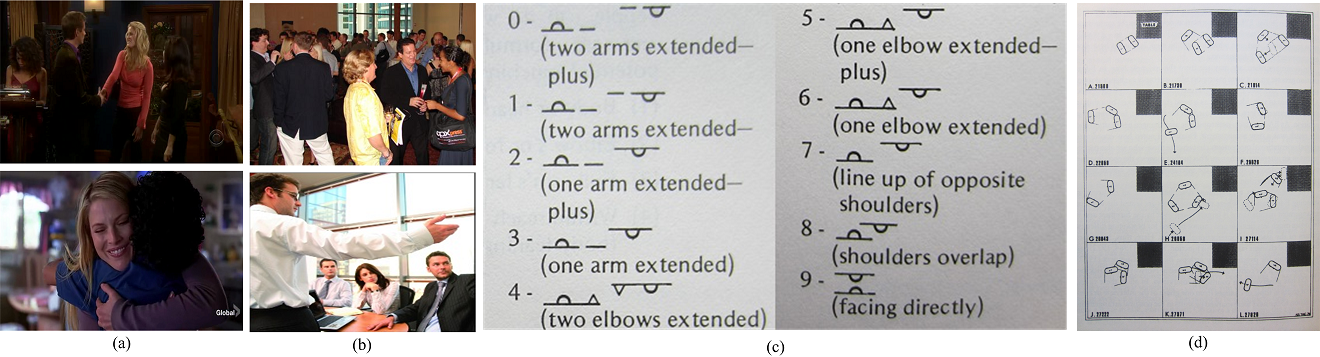
\includegraphics[width=\columnwidth]{socialbehavior_2014}
\end{center}
\vspace{-0.25in} \caption{\captionsize 
Social encounters are ubiquitous (a--b). We will study them and their underlying social relationships by learning and detecting salient, environment-specific ``proxemes" as generalizations of those manually defined by social scientists, such as (c) the body configuration spectrum~\cite{hall1974} and (d) ``f-formations" \cite{Kendon1990}. \label{fig:socialbehavior}\afterfigspace}
\end{figure}


Our goal is to build a computational foundation for inferring the social relationships between every pair of dominant individuals captured in an image/video collection. As stated previously, this will require coordinated innovations in semantic image processing and in signal processing on social graphs. Semantic image processing is required to localizing human targets, compute their attributes, and most novel, detect and recognize their salient elemental interactions (proxemes). Graph signal processing is required to identify unique individuals (nodes), transfer and filter the noisy relationship estimates from target pairs to graph edges, fill in the missing edges due to unobserved co-occurrences, and make joint decisions at all edges about relationship types and strengths.

We will employ off-the-shelf tools to detect and compute attributes (gender, age, and occupation, etc.) of  human targets (e.g.,~\cite{LNCS53050340, Gender, Age}), but the focus of our proposed research will be to develop foundations for new tools that can detect and recognize instances of proxemes---categories of elemental, multi-person interaction units that provide a useful intermediate representation between input imagery and the relationships in the underlying social network. This idea is deeply rooted in the social sciences, where observational studies of human gatherings have repeatedly demonstrated three facts: 1) the nature of visual interactions vary substantially from one setting to the next; 2) within any one setting, customary patterns of visual interaction tend to emerge; and 3) instances of these customary patterns are indicative of the social roles and relationships of the participants~\cite{Kendon1990,kendon1975some,Scherr2009}. Figure~\ref{fig:socialbehavior}(c--d) show two examples of ``proxeme dictionaries'' that have been manually (and painstakingly) defined by social scientists, and there are many others.

\comment{For example, the customary patterns of\comment{head poses, body poses,} poses and gestures\comment{ that emerge} during introductory encounters\comment{ at a cocktail party} are very different from those\comment{ that emerge} in the middle of sustained conversations~\cite{Kendon1990}, and these in turn are very different from the customary patterns for a romantic couple on a park bench~\cite{kendon1975some}, students working around a table~\cite{Scherr2009}, colleagues meeting in a boardroom (Fig.~\ref{fig:socialbehavior}(b)), or students collaborating in comment{ theater-like} lecture hall (Fig.~\ref{fig:prodic}(a)). }

\comment{
These ideas are well-established but, at present, operationalizing them is a phenomenally onerous task. Social scientists must watch and re-watch many filmed specimens of interaction in a particular setting and do their best to manually identify meaningful, recurring patterns. Figure~\ref{fig:socialbehavior}(c--d) shows two successful examples of this, and there are many others; but this manual approach is fundamentally limited by the availability of human experts, their patience, and their abilities to recognize patterns in large image and video datasets. By creating computational representations and methods that emulate this manual process, we seek to establish a framework for data-driven analysis of visual interactions and relationships that can be applied at transformative scales.This effort is timely because of maturing technologies: As described in Sec.~\ref{sec:background}, a variety of serviceable systems exist, and by integrating them one can extract crude but usable descriptors of individual and relative behaviors in the form of positions, trajectories, histograms-of-flow, bags of interest points, and so on. With these types of features, an image can be abstracted as a noisy collection of positional features, and a video can be abstracted as a noisy collection of space-time features.  The performance of this abstraction will continue to increase as these tools continue to evolve. 
}
%(see Fig.~\ref{fig:intro})

Upon detecting and recognizing a pair of image targets as an instance of a socially-informative proxeme, we will be able to obtain an estimate of relationship types---a noisy vector-valued observation---for that pair. We will then develop\comment{ a new suite of} signal processing tools to reconstruct the complete social network among the unique individuals shown in the image/video collection. These tools must address a set of novel challenges. First, a single individual repeatedly appears in multiple images or videos and thus gives rise to multiple detected targets. These co-exist with many other ``background'' targets generated by imperfect face/human detectors and nonparticipating by-standers, and they are only weakly linked by similarity scores that are estimated between every target-pair. Identifying the unique dominant individuals therefore requires robust graph coarsening methods that can distill the massive pairwise target graph to a smaller graph of individuals. Second, relationship information between individuals is noisy and weak, so information must be averaged, by appropriate filters, across the social network graph. This requires a new class of filters, for both denoising and prediction, that can operating on multi-dimensional relationship signals defined on edges (rather than nodes) of the social graph. Third, to make a decision about the type of relationship between each pairs of individuals, one must consider higher-order constraints between relationship types. If A is the sibling of B, for example, and A is the child C, then B must be the niece or nephew of C. This means that we cannot treat the edge dimensions independently, and that we must create multidimensional processes.

\comment{To meet these challenges, we will extend the state-of-art studies on scalar signals defined on the nodes (0-cell) of a fixed known graph, to the case where graph topology must be inferred before signals on edges (1-cell) can be analyzed and processed. New models and algorithms will be developed, in consolidating ideas of statistical machine learning, but more important in deriving from high-level theoretical abstractions in functional analysis on graph or more generic discrete structure \cite{Grady10}.}

\comment{Altogether, we will accomplish the goal in three inter-connected parts: 1) Representing, detecting, and recognizing social proxemes; 2) Robust graph coarsening; and 3) Multi-dimensional signal processing on the graph edges. Simultaneously, we will strive on creating benchmark datasets to evaluate our methods and design challenge problems to engage our colleagues and to enable reproducible research while preserving privacy.} The rest of this section details how we will address each of these challenges, measure our progress, and engage our colleagues in this important research agenda.



\subsection{Proxemes and their Proximity: The Representation Space of Interactions}
\label{sec:activity}
\vspace{-5pt}
Among the semantic image processing tools that are necessary for our goal, the focus of our research program deals with learning environment-appropriate proxeme dictionaries, and detecting occurrences of proxemes in novel imagery. At the most basic level, this requires inventing two things: 1) a computational representation of interactions; and 2) a recipe for measuring the similarity (or distance) between two interactions. When co-developing these two things, we have four desiderata. First, they must be discriminative, meaning that the similarity between instances of distinct proxemes should be low while that for instances of the same proxeme should be high. Second, they must be insensitive to distractors, such as changes in occasional occlusions, \comment{participant identities,}temporal extent, and rates of progression within the interaction. \comment{Third, they must be robust and inexpensive, so that we can automatically process large image collections and long videos of large social gatherings.} Third, they must be inexpensive and flexible, meaning that they should be able to maximally exploit varying levels of image information, from low-resolution surveillance video to high-fidelity photographs. Fourth and finally, they must accommodate interactions that are hard to describe or encode using explicit grammars, such as required by coupled hidden Markov models~\cite{Brand:CHMM,oliver2000bayesian,mccowan2005automatic}.

\comment{
These desiderata motivate a departure from classical approaches to video, such as coupled hidden Markov models~\cite{Brand:CHMM,oliver2000bayesian,mccowan2005automatic}, that are inspired by speech analysis and represent interactions explicitly as structured per-agent event sequences that are interconnected in time. These approaches can provide very robust detection and recognition of certain types of interactions, but before they can be applied one must optimize for each interaction category the connectivity of atomic events within and between the threads as well as their parameters. This is a daunting task that requires hundreds of cleanly-labeled training samples for each category, and it is not clear how it could be adapted to discover/cluster categories when only few or weak annotations are available.
}
To meet these desiderata, we will develop a new class of interaction representations that are better suited to large-scale, data-driven analysis with less supervision. For videos, our simplest representation is based on ensembles of two types of time-varying descriptors: 1) per-agent descriptors that encode the appearance and/or motion of each agent; and 2) relative pairwise descriptors that encode the appearance and/or motion of each agent relative to another. An interaction spanning $T$ time units (frames or handfuls of frames) and containing $M$ (possibly noisy and fragmented) space-time tracks of agents is represented by the ensemble of $M\cdot T$ per-agent descriptors $\mathbf{f}_{m,t}$ and $M\cdot (M-1)\cdot T$ descriptors $\mathbf{g}_{m,m',t}$ for each agent-pair: ${\cal E}=\{\mathbf{f}_{m,t},\mathbf{g}_{m,m',t} \mid t \in \{1\ldots T\}, m,m' \in \{1\ldots M\} \}$. For images, we use the same representation with $T=1$. Computing the similarity between any two interactions amounts to comparing two ensembles ${\cal E}$ and ${\cal E}'$, and detecting new instances of a proxeme amounts to searching through space and/or time for ensembles that are similar to exemplars of that proxeme.

This approach has the advantage of avoiding the explicit description of interaction structure, which is important when an interaction cannot easily be broken down according to any pre-defined grammar, or when one lacks the vocabulary (or aligned and labeled training data) to precisely describe the coupled sequences of per-agent events. It is flexible because the dimension and form of the descriptors $\mathbf{f}$ and $\mathbf{g}$ can be whatever is appropriate for the setting in question, from centroid position and velocity computed from low-resolution surveillance video to more sophisticated descriptors based on space-time interest points, silhouettes, histograms of flow, body pose, expressions, gestures, or higher-level individual action categories. Finally, as we will describe in the remainder of this section, it can be readily combined with matching techniques for comparisons that are insensitive to the distractors described above, allowing us to operationalize the notion of \emph{proxemes} as simple categories of our descriptor-ensembles.








%\comment{In the third part, one should not expect simple one-to-one mappings between proxemes and relationships. Rather, it is the structural distribution of proxemes that matters, in the same way that texton distributions carry information about texture~\cite{leung2001representing} and structured distributions of SIFT descriptors carry information about object and scene categories~\cite{grauman2005pyramid,lazebnik2006beyond}.}



%To the end of our comprehensive framework to sense a social network from visual information, our research agenda on social visual analytics spans two specific major aspects: 1) Detection and recognition of social interaction categories; 2) Social network estimation from multiple visual sources. To facilitate our research activity, we have built up a hardware and software infrastructure as a prototype system and achieved promising preliminary results.

%\begin{figure}[t!]
%\begin{center}
%\includegraphics[width=\columnwidth]{image_feature}
%\end{center}
%\vspace{-0.25in} \caption{\captionsize 
%Socially-informative visual cues from still images: (a-1) Original picture with detected faces; (a-2) relative positions of the detections; (a-3) Facial expressions; (a-4) Relative gazes; (a-5) Relative poses; (a-6) scene recognition. \label{fig:prob1}\afterfigspace}
%\end{figure}

%Images and videos of people reveal information about their interactions, roles, and relationships through a variety cues. The still image in the top-left of Fig.~\ref{fig:intro} suggests the two individuals are friends instead of colleagues because of their proximity, their poses and expressions, and the scene category (restaurant/bar) in which they appear. All of these cues are accessible with varying degrees of certainty using existing tools for face detection, pose and expression estimation, and scene recognition; and their utility for social analysis has already been demonstrated by recent efforts to recover information about age and gender~ \cite{Gallagher}, relationship categories (e.g., father-daughter vs. siblings)~\cite{Wang2010} and event categories (e.g., beach party vs.~country bar)~\cite{Murillo2012}.

%Images and videos of human gatherings reveal information about roles and relationships through the visual interactions they depict. The photograph in the top-left of Fig.~\ref{fig:intro} suggests the two subjects are close friends because of their apparent proximity, their poses and expressions, and the scene (restaurant/bar) in which they appear. All of these cues are accessible with varying degrees of certainty using existing tools for face detection, pose and expression analysis, and scene recognition; and as described in Sec.~\ref{sec:recent-influences}, their utility has already been demonstrated for certain aspects of interaction analysis and social understanding.

%Videos contain even richer information about interactions and relationships. In some cases, this can be accessed simply by choosing from the video one keyframe that allows clearer categorization of the interaction, such as the hand-shaking or hugging in Fig.~\ref{fig:socialbehavior}(a). In other cases, much more may be revealed by the spatio-temporal structure of the actors' behaviors. For example, the video before and after the frames in Figs.~\ref{fig:socialbehavior}(b) would reveal attention-response behaviors, turn-taking behaviors, and relative shifts in body position that indicate changes in mutual engagement.

%\begin{figure}[b]
%\begin{center}
%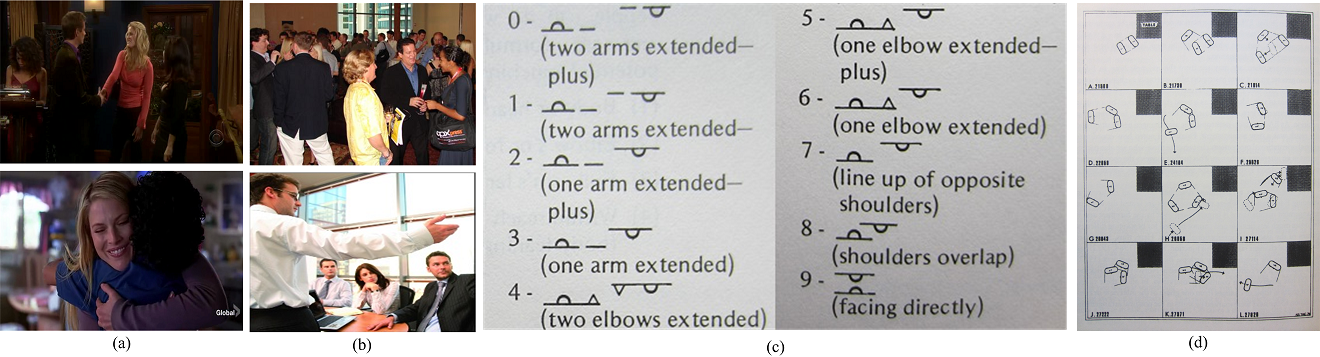
\includegraphics[width=\columnwidth]{socialbehavior_2014}
%\end{center}
%\vspace{-0.25in} \caption{\captionsize 
%Social encounters are ubiquitous (a--b). We will study them and their underlying social relationships by learning and detecting salient environment-specific ``proxemes" as generalizations of those studied in social science (e.g., body %configuration spectrum (c) \cite{hall1974} and ``f-formations" (d) \cite{Kendon1990}) in new environments. 
%(a): Socially non-informative co-occurrence of articulations\cite{UTdata}; (b): Socially non-informative collective crowd activities\cite{Choi:context,Choi:recogtrack,WangMG09}; (c)(d): Socially informative salient interactions; (e) Socially meaningful three-way activity categories defined as `f-formations' by sociology\cite{Kendon1990}.
%\label{fig:socialbehavior}\afterfigspace}
%\end{figure}


%Our goal is to build a computational foundation for social visual analysis by creating tools for extracting as much information as possible about interactions and relationships between people. Our methods will apply to both images, for which social analysis is somewhat established, and videos, for which social analysis is in its infancy; and they will incorporate social interaction categories as a useful intermediate representation between input imagery and the underlying social network. For example, if two individuals are detected as frequently participating in a collegial one-on-one conversation around the water cooler at their workplace, their relationship is likely to be friendly in addition to professional. Similarly, if we observe attention-response instead of turn-taking in a meeting or conversation (Figs.~\ref{fig:socialbehavior}(c--d)) we can recover more detailed information about the interactions and relationships between friends and colleagues.

%Our goal is to build a computational foundation for social visual analysis.  Our approach is based on the idea that dictionaries of \emph{proxemes}---or categories of elemental, multi-person interaction units---provide a useful intermediate representation between input imagery and the underlying social network. This idea is deeply rooted in the social sciences, where observational studies of human gatherings have repeatedly demonstrated three facts: 1) the nature of visual interactions vary substantially from one setting to the next; 2) within any one setting, customary patterns of visual interaction tend to emerge; and 3) instances of these customary patterns are indicative of the social roles and relationships of the participants. For example, the customary patterns of head poses, body poses, and gestures that emerge during introductory encounters at a cocktail party are very different from those that emerge in the middle of sustained conversations~\cite{Kendon1990}, and these in turn are very different from the customary patterns for a romantic couple on a park bench~\cite{kendon1975some}, students working around a table~\cite{Scherr2009}, colleagues meeting in a boardroom (Fig.~\ref{fig:socialbehavior}(b)), or students collaborating in a theater-like lecture hall (Fig.~\ref{fig:prodic}(a)). But in all cases, there are customary behavioral units that emerge, and the enumerated instances these units---or proxemes as we call them---carry valuable information about the social roles and relationships of those participating.

%These ideas are well-established but, at present, operationalizing them is a phenomenally onerous task. Social scientists must watch and re-watch many filmed specimens of interaction in a particular setting and do their best to manually identify meaningful, recurring patterns. Figure~\ref{fig:socialbehavior}(c--d) shows two successful examples of this, and there are many others; but this manual approach is fundamentally limited by the availability of human experts, their patience, and their abilities to recognize patterns in large image and video datasets. By creating computational representations and methods that emulate this manual process, we seek to establish a framework for data-driven analysis of visual interactions and relationships that can be applied at transformative scales.

%Our tools for social visual analysis will apply to both images and videos, and we will develop them in three inter-connected parts: 1) tools for learning and representing dictionaries of environment-specific proxemes; 2) tools for detecting and recognizing instances of these proxemes within larger image and video collections; and 3) tools for using proxeme counts and noisy identities to draw inferences about the underlying social network. \comment{In the third part, one should not expect simple one-to-one mappings between proxemes and relationships. Rather, it is the structural distribution of proxemes that matters, in the same way that texton distributions carry information about texture~\cite{leung2001representing} and structured distributions of SIFT descriptors carry information about object and scene categories~\cite{grauman2005pyramid,lazebnik2006beyond}.}The research we propose is timely because of maturing technologies for detecting and tracking the faces and bodies of people and recognizing their identities. As described in Sec.~\ref{sec:background}, a variety of serviceable systems exist, and by integrating them one can extract crude but usable descriptors of individual and relative behaviors in the form of positions, trajectories, histograms-of-flow, bags of interest points, and so on. With these types of features, an image can be abstracted as a noisy collection of positional features, and a video can be abstracted as a noisy collection of space-time features (see Fig.~\ref{fig:intro}). Our goal is to enable the automatic recovery of useful social based on the features that are available \emph{today}, with the understanding that performance will automatically increase as these tools continue to evolve. Our principal challenge, therefore, is to distill useful information from the substantial and unavoidable uncertainties caused by false detections, broken tracks, noisy features, and erroneous proxeme recognitions. The rest of this section details how we will address these challenges, measure our progress, and engage our colleagues in this important research agenda.

%For example, if two individuals are detected as frequently participating in a collegial one-on-one conversation around the water cooler at their workplace, their relationship is likely to be friendly in addition to professional. Similarly, if we observe attention-response instead of turn-taking in a meeting or conversation, we can recover more detailed information about the relationships between friends and colleagues.

%In order to recover social information from image data, we propose a broad set of tools that enable: 1) representing the space of social interactions in an environment by a discrete set of environment-specific categories; 2) automatically recording over time and space the rates at which different individuals participate in these interaction categories; and 3) using these recordings along with the image data to draw inferences about the underlying social network. Our proposal is inspired by research in sociology~\cite{Kendon1990,Hoyle,Tannen}, economics~\cite{econo_category}, and education~\cite{Scherr2009}, where various social environments  have been  analyzed in terms of a small numbers of interaction categories that are salient and semantically-meaningful (e.g., conversational ``f-formations''~\cite{Kendon1990} in Fig.~\ref{fig:socialbehavior}(e)). It is also motivated by our preliminary results, which suggest that semantically-meaningful interaction categories can reliably be detected and recognized in a real-world (classroom) setting.

%In order to recover social network from image data, we propose a broad set of tools that enable: 1) representing the space of social interactions in an environment by a discrete set of environment-specific proxemes (categories); 2) automatically recording over time and space the occurrences and participants of these proxemes; and 3) using these recordings along with the image data to draw inferences about the underlying social network. 

%Our proposal is inspired not only by research in social sciences\comment{~\cite{hall1974,Kendon1990,Hoyle,Tannen}, economics~\cite{econo_category}, and education~\cite{Scherr2009}} which have analyzed a small number of salient and meaningful proxemes (e.g., conversational body configurations \cite{hall1974}  in Fig.~\ref{fig:socialbehavior} (c) and ``f-formations''~\cite{Kendon1990} in Fig.~\ref{fig:socialbehavior}(d)), 


%but also by our preliminary results suggesting that these proxemes can reliably be detected and recognized in a real-world (classroom) setting. It is also motivated by our experiments showing that new domain-specific proxemes can be discovered in an unsupervised or semi-supervised manner when data is abundant but domain-expert guidance is lacking. (See Section~\ref{sec:activity})



%, and we seek general methods that can exploit inputs of varying precision. High-quality imagery can provide fine-scale information about expression, while low-quality imagery might provide only coarse estimates of head pose. Our goal is to create general tools that operate in all cases and make use of as much information as is available.


%We begin with learning and recognizing interactions and then discuss inferring social network information in Section~\ref{sec:vis2net}. We describe datasets and challenge problems in Section~\ref{sec:sys}. 

%We propose to learn and detect interaction categories (Section \ref{sec:activity}), in complementary to those companion efforts for still images. We then propose to infer social network from images and videos by leveraging all socially-informative visual patterns including occurrences of interactions as an intermediate representation (Section \ref{sec:vis2net}).

%(b-1) Independently recognizing the two faces: The right face is hard to distinguish between two possible people; (b-2) Recognizing faces using social relationship inferred from (a-1) through (a-6): The right face is now more likely to be associated with one person than the other.

%Consider that in recognizing the two faces detected in Fig. \ref{fig:prob1} (a-1) the right face is hard to distinguish between `Susan' and `Helen' (see (b-1)). However, the inferred `friends' relationship suggests that the individual should belong to the left person's list of friends (see (b-2)), which includes only `Helen' but not `Susan'.

%\subsection{Proxemes and their proximity: The representation space of social interactions}
%\label{sec:activity}

%The first part of our research program deals with learning environment-appropriate proxeme dictionaries, and detecting occurrences of proxemes in novel imagery. At the most basic level, this requires inventing two things: 1) a computational representation of interactions; and 2) a recipe for measuring the similarity (or distance) between two interactions. When co-developing these two things, we have four desiderata. First, they must be discriminative, meaning that the similarity between instances of distinct proxemes should be low while that for instances of the same proxeme should be high. Second, they must be insensitive to distractors, such as changes in viewpoint, participant identities, temporal extent, and rates of progression within the interaction. Third, they must be robust and inexpensive, so that we can automatically process large image collections and long videos of large social gatherings. Fourth and finally, they must be flexible, meaning that they should be able to maximally exploit varying levels of image information,  from low-resolution surveillance video to high-fidelity camera networks.

%These desiderata motivate a departure from classical approaches to video, such as coupled hidden Markov models~\cite{Brand:CHMM,oliver2000bayesian,mccowan2005automatic}, that are inspired by speech analysis and represent interactions explicitly as structured per-agent event sequences that are interconnected in time. These approaches can provide very robust detection and recognition of certain types of interactions, but before they can be applied one must optimize for each interaction category the connectivity of atomic events within and between the threads as well as their parameters. This is a daunting task that requires hundreds of cleanly-labeled training samples for each category, and it is not clear how it could be adapted to discover/cluster categories when only few or weak annotations are available.

%that as an explicit \emph{multi-thread event}~\cite{Hongeng:act} comprised of two or more single-thread events (i.e., two or more temporal sequences of per-person atomic actions) that are

%We propose to develop a new class of representations for social interactions that are better-suited to data-driven analysis, including use of techniques like domain adaptation, active learning, semi-supervised learning, and unsupervised learning, which can help reduce the number of training samples to enable widespread use. Our representations are based on ensembles of two types of time-varying descriptors: 1) per-agent descriptors that encode the appearance and/or motion of each agent; and 2) relative pairwise descriptors that encode the appearance and/or motion of each agent relative to another. In the simplest case, an instance of an interaction spanning $T$ time units (frames) and containing $M$ (possibly noisy and fragmented) space-time tracks of agents---these could be centroid locations, bounding boxes, silhouettes, etc.---is simply represented by the ensemble $\{\mathbf{f}_{m,t},\mathbf{g}_{m,m',t}\}$ of $M\times T$ per-agent descriptors $\mathbf{f}_{m,t}$ and $M\times (M-1)\times T$ per-pair descriptors $\mathbf{g}_{m,m',t}$. Computing the similarity between any two interactions amounts to comparing two ensembles, and detecting an interaction category in a long video of a larger social gather amounts to searching through space and time for ensembles that are similar to one or more exemplars in that category. 

%We will develop a new class of interaction representations that are better suited to large-scale, data-driven analysis with less supervision. For videos, our simplest representation is based on ensembles of two types of time-varying descriptors: 1) per-agent descriptors that encode the appearance and/or motion of each agent; and 2) relative pairwise descriptors that encode the appearance and/or motion of each agent relative to another. An interaction spanning $T$ time units (frames or handfuls of frames) and containing $M$ (possibly noisy and fragmented) space-time tracks of agents is represented by the ensemble of $M\cdot T$ per-agent descriptors $\mathbf{f}_{m,t}$ and $M\cdot (M-1)\cdot T$ descriptors $\mathbf{g}_{m,m',t}$ for each agent-pair: ${\cal E}=\{\mathbf{f}_{m,t},\mathbf{g}_{m,m',t} \mid t \in \{1\ldots T\}, m,m' \in \{1\ldots M\} \}$. For images, we use the same representation with $T=1$. Computing the similarity between any two interactions amounts to comparing two ensembles, and detecting new instances of a proxeme amounts to searching through space and/or time for ensembles that are similar to exemplars of that proxeme.

%Our ensemble-based approach has the advantage of avoiding the explicit semantic description of social interactions, which is important when an interaction category cannot easily be broken down according to any pre-defined grammar, or when one lacks the vocabulary to precisely describe the coupled sequences of atomic events that comprise it. It is flexible because the dimension and form of the descriptors $\mathbf{f}$ and $\mathbf{g}$ can be whatever is appropriate for the setting in question, from centroid position and velocity computed from low-resolution surveillance video to more sophisticated descriptors based on space-time interest points, histograms of flow, body pose, expressions, gestures, or higher-level individual action categories. Finally, as we will describe in the remainder of this section, it can be readily combined with matching techniques for comparisons that are insensitive to distractors, allowing applications from learning to detection and recognition.

%Our ensemble-based approach has the advantage of avoiding the explicit semantic description of interactions, which is important when an interaction cannot easily be broken down according to any pre-defined grammar, or when one lacks the vocabulary (or aligned and labeled training data) to precisely describe the coupled sequences of atomic events. It is flexible because the dimension and form of the descriptors $\mathbf{f}$ and $\mathbf{g}$ can be whatever is appropriate for the setting in question, from centroid position and velocity computed from low-resolution surveillance video to more sophisticated descriptors based on space-time interest points, silhouettes, histograms of flow, body pose, expressions, gestures, or higher-level individual action categories. Finally, as we will describe in the remainder of this section, it can be readily combined with matching techniques for comparisons that are insensitive to the distractors described above, allowing us to operationalize the notion of \emph{proxemes} as simple categories of our descriptor-ensembles.

%More precisely,  specifically, assume an input video consisting of $T$ frames. By applying domain-appropriate detection and tracking, assume we obtain $M$ space-time tracks of bounding boxes enclosing $M$ faces or bodies. The $M$ targets are to be compared with an interaction exemplar consisting of $S$ frames and $N$ targets ($N\le M$) that are correctly detected and tracked and all participating in an coherent interaction. Our representation for the input tracks therefore includes $M\times T$ $d_{I}$-dimensional descriptors $\{\mathbf{f}_{m,t}\}_{m=1,2,\cdots,M, t=1,2,\cdots,T}$, where $\mathbf{f}_{m,t}$ encodes the individual activity of the $m$th target at time $t$, and $M\times (M-1)\times T$ $d_{P}$-dimensional pairwise descriptors $\{\mathbf{g}_{m,m',t}\}_{m,m'=1,2,\cdots,M, m\neq m', t=1,2,\cdots,T}$, where $\mathbf{g}_{m,m',t}$ encodes dynamic visual properties of target $m$ exhibited relative to those of target $m'$ at time $t$. Meanwhile, the the interactions of interest are stored as exemplars in a gallery, each exemplar associated with a category label. For each exemplar, we have two similar descriptor collections $\{\mathbf{f}^{D}_{n,s}\}_{n=1,2,\cdots,N, s=1, 2,\cdots, S}$ and $\{\mathbf{g}^{D}_{n,n',s}\}_{n,n'=1,2,\cdots,N, n\neq n', s=1, 2,\cdots, S}$. We denote the descriptor ensemble for the input at time $t$ to be $\mathcal{Q}_{t}\triangleq\{\mathbf{f}_{m,t},\mathbf{g}_{m,m',t}\}$, and that for the exemplar at time $s$ as $\mathcal{D}_{s}\triangleq\{\mathbf{f}^{D}_{n,s},\mathbf{g}^{D}_{n,n',s}\} $. The input is then represented as $\mathcal{Q}\triangleq\{\mathcal{Q}_{t}\}_{1\leq t\leq T}$ and the exemplar $\mathcal{D}\triangleq\{\mathcal{D}_{s}\}_{1\leq s\leq S}$. We show that the can allow efficient measurement of distance in Section \ref{subsec:activity}, and then describe how it serves as a foundation for learning interaction categories in Section \ref{sec:actlearn}.


%We seek to develop new approaches for detecting, localizing, and recognizing these socially informative visual patterns, i.e., interactions, from videos, in complementary to those companion efforts for still images. Through this effort, we foresee a richer set of heterogenous socially informative visual cues from videos in addition to those from images, so as to enable high-level reasoning as to be introduced in Section \ref{sec:vis2net}. 
%We propose a paradigm as to be detailed in Section \ref{subsec:activity}, which is different from the existing work in three aspects. 

%Second, we propose to predict activities under social contexts. In this case, social semantics assist in visual understanding in the way that they serve as contextual information for restricting the more possible categories of activities that may occur between a specific group of individuals. This effort is also complementary to the usage of social contexts for identifying the targets presented in the previous section. Consider a simple illustrative example in which we would like to label a conversational scene in a movie as either a `negotiation� or a 'debate'. It is possible, in this case, that by the analysis of facial expressions, gestures, and poses, we still have difficulty in distinguishing the two. However, by appropriate face recognition in association with other metadata of the movie, probably with the help of social contexts as introduced in the previous section, we may gain solid confidence regarding the social relationship between the speakers as either `cooperative' or 'adverse'. A cooperative relationship are more likely to imply a negotiating activity, and an adverse relationship implies otherwise. A mechanism, similar to and in companion to the CRF formulation but adapted to video analysis, will be particularly useful.

%
%In our following research, we aim to enrich the descriptions of the social behaviors in the current prototype system, explore more accurate and robust comparison and retrieval mechanisms, and in particular, design novel modules for integrating social contextual annotations to allow our framework to be fully `socially-aware'.


%%%%%%%%%%%%%%%%%%%%%%%%%%%%%%%%%%%%%%%%%%%%%%%%%%%%%%%%%%%%%%%%%%%%%%%%%%%%%%%%%%%%%%%%%%%%%%%%%%%%%%%%%

%\subsection{Joint Recognition of Multiple Targets with Social Contexts}
%\label{sec:recognition}
%
%The automatic recognition of targets in image and videos is an central task of computer vision. Recognition of objets is not only essential to any system that seeks to manage visual media based on content, but also necessary for automatically annotating images/videos (`auto-tagging') and indexing them. Recognition of faces is even integral to successfully interpreting images/videos of humans and consequently mining the social semantics in these imagery.
%
%Automatic recognition, since its initial stage until most recently, treats the targets as well as the outputted categories to be independent rom one to the other, which is essentially not the case. In order for automatic recognition to truly succeed, we must exploit the syntactic relationships between targets and between categories and use other contextual information. We in this section propose a scalable computational framework for socially-aware recognition systems that exploit contextual information from online social networks. These online communities provide two significant types of information which, to date, have only been scarcely exploited: 1) significant textual metadata, and 2) social network structure as context. The proposed activity seeks computational foundations for exploiting both.
%
%A typical example of socially-aware face recognition is as follows. A user uploads a small, hundred-image `album' (say)  and we seek to automatically recognize the identities of detected faces in the images. To achieve this goal, we represent the detected faces as nodes in a densely connected, undirected graph. With this representation, recognition consists of estimating a joint labeling of the nodes, which can be formulated as the optimization of an energy-based model. What is unique to our approach is that we seek energy models that combine image information (e.g., classifier output) with contextual information drawn from the user's online social network. Another example is scene recognition, where we seek to jointly label all images with their scene categories in several related online album containing thousands of scene images. Similar examples are more than the two mentioned examples.
%
%The description of an individual target is generally in multiple `views', where a view refers to a specific type of attribute that describes the target. A detected face, for example, can be described by skin color, texture, shape configurations of facial organs, etc.. The description of the contextual network relationship, meanwhile, is also in multiple views. The context between two faces(humans) in Facebook, for example, can be number of their shared friends, the number of their co-occurrence, and their relative poses in images, and so on. As we have mentioned, the social networks are usually partially observed, meaning that not all these views are `visible', and a practically useful recognition system must accommodate the un-observed views for the nodes or the links. Formally,  we can represent  the densely connected, undirected graph as $G$ describing the community of $K$ individuals, where $G\triangleq\{N^{(v_1)},A^{(v_2)},P^{(v_1)}, Q^{(v_2)}\}, v_1=1,2,\cdots,V_1,\hspace{5pt} v_2=1,2,\cdots,V_2$,  $N^{(v_1)}$ is a $K\times 1$ vector describing the individuals in the $v_1$th view, $P^{(v_1)}$ is a $K\times 1$ binary vector describing the visibility for that view, $A^{(v_2)}$ is the $K\times K$ affinity matrix describing the relational context for the $v_2$th view, and $Q^{(v_2)}$ is the $K\times K$ visibility matrix for that view. If $P^{(v_1)}(i)=1$, then $N^{(v_1)}(i)$ is the scalar description of the individual $i$ in the $v_1$th view; otherwise if $P^{(v_1)}(i)=0$ then $N^{(v_1)}(i)$ is a missing number indicating the lack of information of this node in this view. Similar notions apply for the matrices $A$ and $Q$.
%
%With this formulation, a natural computational framework for this socially-aware recognition is a conditional random field (CRF) model~\cite{lafferty2001crf, sutton2007icr, he2004mcr} with a node for each item of interest and an edge connecting many pairs of nodes. In this case, the goal is to infer a joint labeling $\vy=\{y_i\}$ of the relevant categories over all nodes $i$ in the graph. We use the notation $y_i\in{\cal L}=\{l_0\ldots l_M\}$ for the discrete label space of the nodes. (In general, these will vary from node to node, but we use a single set of labels here for notational convenience.) An optimal joint labeling is found by maximizing the conditional density
%\begin{equation} \label{eq:crf}
%{\rm Pr}(\vy|G) = \frac{1}{Z(G)}e^{-E(\vy|G)}
%\end{equation}
%where the partition function $Z(G)$ is a data-dependent normalizing constant and the energy $E(\vy|G)$ consists of sums of unary and pairwise potential functions at the nodes and edges:
%\begin{equation}\label{eq:energy}
%E(\vy|G) =  \sum_{i}  \phi_i (y_i|G) + \sum_{(i,j)} \phi_{ij}(y_i, y_j|G).
%\end{equation}
%
%In the CRF framework, the unary potential functions $\phi_i(y_i|G)$ capture information that is local to each node, and the pairwise potentials $\phi_{ij}(y_i, y_j|G)$ represent the compatibilities of possible label pairs across an edge. Therefore, assuming that the unary potentials depend on individual descriptions and pairwise potentials depend on contextual descriptions, (\ref{eq:energy}) can be decomposed as
%\begin{equation}\label{eq:energy_simple}
%E(\vy|G) =  \sum_{i}  \phi_i (y_i|N,P) + \sum_{(i,j)} \phi_{ij}(y_i, y_j|A,Q).
%\end{equation}
%As part of the proposed activity, we will study the application of this model to practical recognition tasks. Our goal is to answer the following three questions: 1) what types of social network context information improve recognition and by how much?; 2) how should multiple-view of information be weighted and how should missing observation be accounted for?; and 3) how can we apply this model at a practical scale? 
%
%\begin{figure}[t!]
%\begin{center}
%\includegraphics[width=3.5in]{ivw_facescores}
%\end{center}
%\vspace{-0.25in} \caption{\captionsize 
%The performance of a commercial face recognition system on tagged faces harvested from Facebook~\cite{Stone2008}. Given the query face in the upper left, the system has returned the remaining faces as being most similar. Similarity to the query decreases from left to right and from top to bottom, and the ground-truth matches are highlighted with green squares. Due to the variability of this `real-world' dataset, the correct matches are not highly ranked.\label{fig:face-results}\afterfigspace}
%\end{figure}
%
%
%
%\SubSubSection{Preliminary Study}\label{sec:prelim-face-results}
%Evidence for the utility of social network context is provided under simplified assumptions by the work of PI Zickler~\cite{Stone2008,Stone2010}, the former of which received the Best Paper Award at the First IEEE Workshop on Internet Vision. This work reported the results of a preliminary study on the ability of social network context to improve face-based identity recognition using a subset of 2641 labeled faces from Facebook. In this study, we restricted our attention to images with two faces (two-node graphs) so that CRF training and inference could be achieved without approximation. The label space ${\cal L}=\{l_0,\ldots,l_M\}$  consists of a set of possible identities, and we considered a simple set of individual node descriptions and contextual relationship descriptions. Specifically, we assumed that all descriptions in all views are observed and error-free, in which case the potentials in (\ref{eq:energy_simple}) are further expanded as a linear combination of view-specific univariate and bivariate \emph{feature functions} independent of observability variables $P,Q$:
%\begin{eqnarray}
%\phi_i(y_i|N,P) &=& \sum_{v_1} \alpha_{v_1}(N^{(v_1)}) f_{v_1}(y_i, N^{(v_1)})\\
%\phi_{ij}(y_i, y_j|A,Q) &=& \sum_{v_2} \beta_{v_2}(A^{(v_2)}) g_{v_2}(y_i, y_j, A^{(v_2)}).
%\end{eqnarray}
%
%
%\begin{figure}[t!]
%\begin{center}
%\includegraphics[width=5in]{rank_graph_small}\\
%{\footnotesize
%\begin{tabular}{ll}
%\hline\hline\multicolumn{2}{l}{\raisebox{-0.1in}{Univariate Functions $f_{v_1}(y_i, N^{(v_1)})$}} \\
%\hline
%\parbox[t]{1.8in}{\raggedright Face score (\textsf{face})} & \parbox[t]{3.5in}{A distribution of likelihoods over ${\cal L}$ returned by a commercial face recognition system (see Fig.~\ref{fig:face-results})} \vspace{0.03in}\\
%\parbox[t]{1.8in}{\raggedright Photo history (\textsf{hist})} & \parbox[t]{3.5in}{Number of times each individual $l_m$ has been tagged in previous photos posted by the photographer} \vspace{0.07in}\\
%\multicolumn{2}{l}{Bivariate Functions $ g_{v_2}(y_i, y_j, A^{(v_2)})$} \\
%\hline
%\parbox[t]{1.8in}{\raggedright Friendship (\textsf{friend})}& \parbox[t]{3.5in}{Binary indicator that is one iff individuals $l_m$ and $l_n$ are `Facebook friends' } \vspace{0.04in}\\
%\parbox[t]{1.8in}{\raggedright Pairwise co-occurrence (\textsf{pair})}& \parbox[t]{3.5in}{Number of times each pair of individuals $(l_m,l_n)$ has been jointly tagged in previous photos posted by the photographer}\\
%\end{tabular}}
%\end{center}
%\captionspace \caption{\captionsize 
%Face recognition performance as a function of rank threshold for a variety of combinations of feature functions (described bottom). At each rank value $R$, the graph displays the proportion of all test samples for which the correct ground-truth identity label appeared in the top $R$ predictions. Social network context improves recognition, and different sources of context information are complimentary\cite{Stone2008}.\label{fig:ivw-curves}\afterfigspace}
%\end{figure}
%
%
%The results are summarized in Figs.~\ref{fig:face-results} and \ref{fig:ivw-curves}. For each combination of feature functions, we determined model parameters ($\alpha$ and $\beta$) by maximizing the conditional log-likelihood of a training set by gradient ascent. Then, for each left-out test photo, exact marginal probabilities were computed for the test photo's face-nodes, and  the outputs were compared against ground truth. Specifically, the marginal probabilities were used to compute a ranked list at each node, and we measured how often the correct identity label appeared in the top $R$ ranks for a sliding value of $R$ (c.f.~\cite{frvt06}).
%
%A number of observations can be drawn from these results. First, even when using the face score (\textsf{face}) alone (see Fig.~\ref{fig:face-results}) social network context plays a vital role. In our data, over 99\% of tagged faces correspond to `friends' of the photographer, and since the identity of the photographer is known (it is included in the input $N$), we can safely reduce the label space ${\cal L}$ from the 15,752 individuals in the global gallery to the hundreds of friends of the input photographer. Without this restriction, the results in Fig.~\ref{fig:face-results} would degrade remarkably. The results in Fig.~\ref{fig:ivw-curves} also demonstrate that social network context substantially improves baseline face recognition, and that different sources of context information are complementary.
%
%
%These preliminary results are encouraging, especially since the network context information that was employed barely scratches the surface of possibilities. Existing work shows that clothing can provide useful information within an album~\cite{anguelov2007cir, zhang2003aah,  song2006cah, sivic2006fpr}, and it is possible that clothing could be used more globally as well, since the long-term clothing trends of certain individuals may be distinguishable from those of others. Recognition of facial attributes~\cite{LNCS53050340}, such as glasses or facial hair, can be used in conjunction with identity scores to improve recognition, and the same is true for gender recognition, which in many online communities is a knowable piece of information. In addition, people associate with each other in homes, schools, outdoors, workplaces, clubs, and so on, and a more explicit representation of these would be beneficial. Certain individuals will appear more often in certain types of scenes, and these `likely' scene types will change depending on who they are with. Temporal and geographic information, when available, may be further predictive of which individual is likely to occur and with whom. 
%
%
%
%In our proposed research, we aim to both qualitatively and quantitatively analyze large collections of images and their embedding network to discover the utility of these multi-view context information, and in particular, explore effective approaches to account for incompletely observed graph, which is the crucial to allow our framework to succeed in realistic network conditions.
% !TEX root = SocialVision2014.tex
\vspace{-5pt}
\subsubsection{Spatio-Temporal Detection and Classification of proxemes}
\label{subsec:activity}
\vspace{-5pt}

The task of learning a proxeme dictionary will be discussed in the next section. For now, let us assume that the dictionary of proxemes, each of which represented by one of more of its exemplars (i.e., representative descriptor-ensembles from one or more interaction categories), are available, and consider the problem of detecting and recognizing new instances of these proxemes in long videos of large social gatherings. We begin by describing a preliminary system reported recently by the PIs~\cite{groupdet2013}. In this system, proxemes are represented by one or more exemplars, and detecting and recognizing new instances of these proxemes is formulated a matching problem, illustrated in Figure~\ref{fig:proxeme_det_recog} and depicted in more detail in the Figure 1 of~\cite{groupdet2013} \footnote{\url{http://gvi.seas.harvard.edu/sites/all/files/Li_Porfilio_Zickler_CVPR2013.pdf}}. We have an exemplar ${\cal E}=\{\mathbf{f},\mathbf{g}\}$ involving $N$ participants over some interval of time, and we wish to localize within a long video of a larger social gathering ($M>N$ actors) the times and locations in which $N$-agent sub-groups participate in similar interactions. To succeed, we must deal with some of the $M$ tracks being artifacts caused by false detections, and others being fragmented due to tracking breakdowns and agent exits. We must also account for interactions occurring over different temporal extents and at variable rates within their extents.

\begin{figure}[t!]
\begin{center}
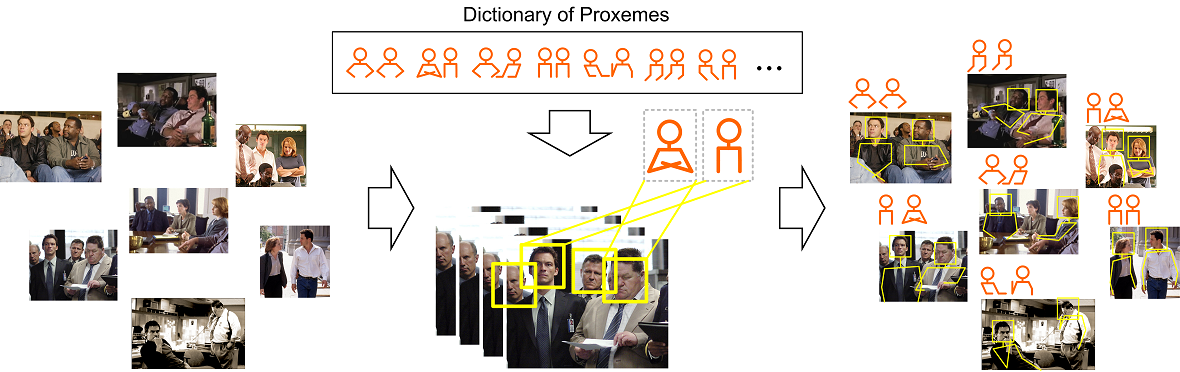
\includegraphics[width=0.75\columnwidth]{proxeme_det_recog}
\end{center}
\vspace{-0.25in} \caption{\captionsize 
Semantic image processing for detecting and classifying proxemes (detail of Fig.~\ref{fig:intro}). We possess one or more exemplars for each proxeme in a proxeme dictionary, and given an input image or video, we must detect salient interactions and associate each detection with its corresponding proxeme. \label{fig:proxeme_det_recog}\afterfigspace}
\end{figure}



To deal with these various sources of noise and outliers, we start with each frame of the exemplar being separately compared to each frame of the long input video, and for each comparison we find the optimal partial matching between the $N$ exemplar participants and the $M>N$ input tracks. Each frame-wise partial match is represented by an $N\times M$ binary matrix $W$ that has at most one non-zero entry in each row and column. \comment{Because our descriptor-ensembles include only unitary and pairwise descriptors}Then, each partial match can be found efficiently using a quadratic program\comment{ similar to that used in shape matching \cite{Berg05shapematching}} $\text{arg}\min_{W=\{w_{nm}\}} \sum_{nm}w_{nm}d_{I}(\mathbf{f}_{m}, \mathbf{f}_{n})+\!\!\!\sum_{nmn'm'}\!\!\!w_{nm}w_{n'm'}d_{P}(\mathbf{g}_{m,m'}, \mathbf{g}_{n,n'})$, where $\{\mathbf{f}_{n},\mathbf{g}_{n,n'}\}$ is the collection of descriptors from one exemplar frame and $\{\mathbf{f}_{m},\mathbf{g}_{m,m'}\}$ is that from one input frame. We can explore many different ``atomic'' distances $d_I,d_P$, and so far we have experimented with one flexible and convenient choice based on Mahalanobis distance: 
\begin{equation}\label{eq:partial-matching}
d_{I}(\mathbf{f}, \mathbf{f}')=(\mathbf{f}-\mathbf{f}')^{T}\Sigma_{I}(\mathbf{f}-\mathbf{f}'), d_{P}(\mathbf{g}, \mathbf{g}')=(\mathbf{g}-\mathbf{g}')^{T}\Sigma_{P}(\mathbf{g}-\mathbf{g}')
\end{equation}
with positive semi-definite matrices $\Sigma_{I}$ and $\Sigma_{P}$ that are data-optmized. Having computed all per-frame partial matches between the frames in exemplar ${\cal E}$ and the input video, we employ a sliding window approach that sequentially considers all temporal windows of the input video (with each temporal window $\mathbf{w}$ represented by its descriptor ensemble ${\cal E}_\mathbf{w}$) and: 1) makes a robust decision about the locations of the $N$ best-matching participants in each temporal window by accumulating weighted votes (in the discrete space of all possible $W$ matrices) from the relevant frame-wise matches; 2) optimally refines the start and end points of the window $\mathbf{w}$ using an efficient branch-and-bound search; and 3) ultimately returns a similarity score $S({\cal E},{\cal E}_\mathbf{w})$. We have evaluated the proxeme detection and classification approach using an early precursor to the Harvard Interactive Classroom Dataset that will be described in Section~\ref{sec:sys}. Our results are detailed in~\cite{groupdet2013}, and they show that this preliminary system not only provides useful performance on this challenging classroom dataset, but also achieves state-of-the-art performance on simpler, standard benchmark datasets involving both humans~\cite{UTdata} and animals~\cite{CRIM13}, demonstrating robustness to false detections and insensitive to moderately broken tracks. 

This functionality of detecting an interaction and associating it with a proxeme instance naturally enables the estimation of the social relationship between the two images targets. As long as the exemplar ${\cal E}$ represents a proxeme that is strongly associated with particular social relationships, it will cast a distribution over relationship-types for the interacting targets involved in ${\cal E}_\mathbf{w}$. (For us, relationship-salient proxemes will include those defined by social scientists~\cite{hall1974,Kendon1990,kendon1975some,Scherr2009} as well as those we will discover from data as described in~\ref{sec:actlearn}.) Denoting the involved targets as $m$ and $n$, the probability $z_{mn}(k)$ of the $k$-th type of relationship between them serves as the input to relationship filtering and network reconstruction as described in \ref{sec:vis2net}. More importantly, the approach also provides a foundation for unsupervised learning of proxemes from data, because it provide a way to compute the similarity $S({\cal E},{\cal E}')$ between any two interaction specimens represented by ensembles ${\cal E}$ and ${\cal E}'$, as discussed in~\ref{sec:actlearn}.





\comment{Through a combination of face detection and tracking, we obtained noisy tracks for all agents and computed simple descriptors based on absolute and pair-wise relative head poses. With input from educational experts we manually defined seven semantically-meaningful proxemes based on head poses, and we manually annotated the participants and temporal extents of 366 distinct instances of these proxemeswithin a much larger video corpus that includes dozens of students observed over many camera-hours. The exemplar interactions range from a few seconds to tens of seconds in length, and the number of by-standers in a video is much larger than the number of participants ($M$ is between 10 and 20 while $N=2,3$).}



\boldstart{Future directions}. While these early results are promising, they are but a small indication of what is achievable. We will explore a number of new representations and similarities for interactions. This includes matching algorithms for higher-order descriptor-ensembles, with relative, between-agent descriptors defined not just pairwise but between three- or four-agent cliques, and between each agent and the entire group. We will also explore similarities that incorporate loose and flexible models for the spatial and temporal structure within a descriptor-ensemble, as space-time analogies to what has proven useful for part-based object and scene recognition~\cite{lazebnik2006beyond,pictorial1973,DPM2013} \comment{ the loose spatial models that have been successful for recognizing scene categories based on distributions of quantized local interest points, and to flexible parts-based models for recognizing object categories}. We will also explore measures of interaction similarity that, instead of being designed for category recognition, are specifically designed as a means to compute ``interaction intensity'' in space and time, as analogous to measures of ``objectness'' proposed for photographs~\cite{alexe2012measuring}.

We will also enhance the domain-specific proxeme dictionaries and their associated social semantics. We will develop mechanisms for data-driven discovery of salient proxemes in a new image set or domain where expert knowledge is scarce or unavailable, as enabled by the computable similarity $S({\cal E},{\cal E}')$ and approaches to be introduced next. Very critically, we will enrich the preliminary set of social relationship types considered in earlier social science studies, and bring in a comprehensive taxonomy of relationship categories to associate with the proxeme categories. This taxonomy will be borrowed, for example, from ``WordNet" \cite{MillerWordNet}, a large lexical database of words that are grouped into sets of cognitive synonyms (synsets), each expressing a distinct concept and that has been employed by various semantic annotation tasks \cite{TouschSHI}. The taxonomy will provide the set of relationship types, indexed by $k$ in the probability $z_{mn}(k)$, which will be transferred to the social graph edges through the associated salient proxeme as to be discussed in~\ref{sec:vis2net}.








%\begin{wrapfigure}{r}{0.5\textwidth}
%\vspace{-20pt}
%  \begin{center}
%    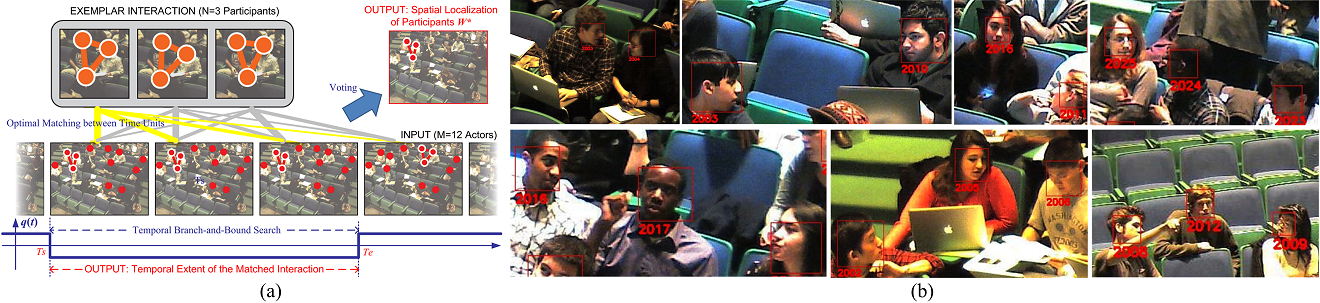
\includegraphics[width=0.5\textwidth]{groupdet2013}
%  \end{center}
%  \vspace{-20pt}
%  % \caption{Preliminary system for detecting and recognizing social proxemes using the proposed representation.}
%  % \vspace{-15pt}
%%\label{fig:diagram}
%\end{wrapfigure}




%We approach detection and recognition as a matching problem, depicted in the left of Fig.~\ref{fig:diagram_dataset}. Suppose we have an exemplar from an interaction category involving $N$ participants, and we wish to localize within a long video of a larger social gathering ($M>N$ tracks) the times and locations in which sub-groups of agents participate in similar interactions. To succeed, we must deal with some of the $M$ tracks being artifacts caused by false detections, and others being fragmented due to tracking breakdowns and agent exits. We must also account for interactions occurring over different temporal extents and at variable rates within their extents.



%\begin{figure}[t!]
%\begin{center}
%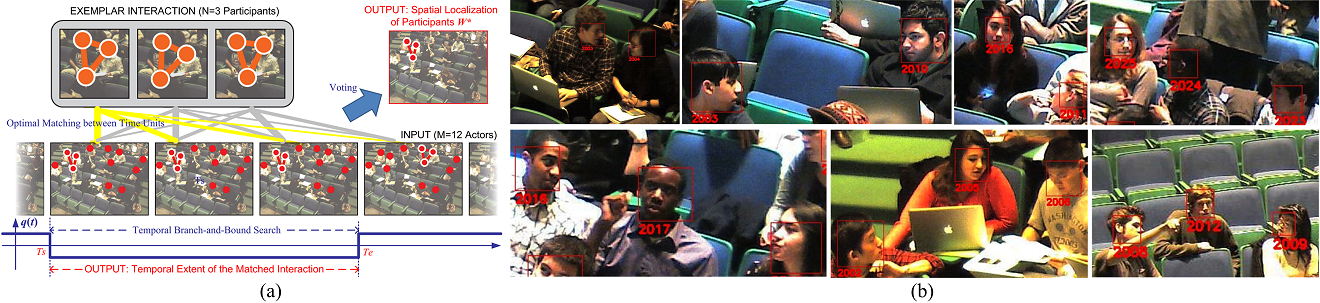
\includegraphics[width=\columnwidth]{groupdet2013}
%\end{center}
%\vspace{-0.25in} \caption{\captionsize 
%(a): Preliminary system for detecting and recognizing social proxemes using the proposed representation. (b): Examples of the educationally-meaningful proxemes.}
%\label{fig:diagram_dataset}\afterfigspace
%\end{figure}



%where $\{\mathbf{f}_{n},\mathbf{g}_{n,n'}\}$ is the collection of $N$ individual and $N\times (N-1)$ pairwise descriptors from one exemplar frame and $\{\mathbf{f}_{m},\mathbf{g}_{m,m'}\}$ are the $M$ and $M\times (M-1)$ individual and pairwise descriptors from one frame of the input. 

%\todd{Working here}. To formally describe task consider the fact that if one of the $M$ targets is regarded as a participant in an interaction as exemplified by the exemplar $\mathcal{D}$, its behavior should properly match to the behavior of one of the $N$ individuals in the exemplar $\mathcal{D}$. Therefore, we use a $N\times M$ binary matrix $W=[w_{nm}]\in\{0,1\}^{N\times M}$ to formally represent the participant identification, where $w_{nm}=1$ means that the $n$th exemplar individual is matched to the $m$th input target and $w_{nm}=0$ means unmatched targets. For unambiguous matching, we expect each individual in the exemplar to find its unique partner target in the input. This implies that $\sum_{m}w_{nm}=1, \forall n$ and $\sum_{n}w_{nm}\leq 1, \forall m$, \textit{i.e.}, $W\mathbf{1}=\mathbf{1}$ and $\mathbf{1}^{T}W\leq\mathbf{1}^{T}$. Denote $\mathcal{W}\triangleq\{W\in\{0,1\}^{N\times M}| W\mathbf{1}=\mathbf{1}, \mathbf{1}^{T}W\leq\mathbf{1}^{T}\}$, and our former task is essentially to find $W^{*}\in\mathcal{W}$, which encodes the best matching between the input $\mathcal{Q}$ and the exemplar $\mathcal{D}$. To formally describe task 2) is straightforward: We simply look for the starting time $T_{s}$ and ending time $T_{e}$, $1\le T_{s}<T_{e}\le T$, such that the interactive pattern of input $\mathcal{Q}$ during $[T_{s}, T_{e}]$ demonstrates the best similarity with the exemplar $\mathcal{D}$.


%Suppose that there are Mahalonobis-parameterized atomic distances $d_{I}(\mathbf{f}, \mathbf{f}')=(\mathbf{f}-\mathbf{f}')^{T}\Sigma_{I}(\mathbf{f}-\mathbf{f}')$ and $d_{P}(\mathbf{g}, \mathbf{g}')=(\mathbf{g}-\mathbf{g}')^{T}\Sigma_{P}(\mathbf{g}-\mathbf{g}')$ ($\Sigma_{I}\succeq 0$ and $\Sigma_{P}\succeq 0$ are positive semi-definite matrices) to compare descriptors, and accordingly define the `instantaneous' matching between input $\mathcal{Q}_t$ and exemplar $\mathcal{D}_s$ under matrix $W$ can be defined as 
%\begin{equation}
%\hat{D}(\mathcal{Q}_{t}, \mathcal{D}_{s}, W)=\sum_{nm}w_{nm}d_{I}(\mathbf{f}_{m,t}, \mathbf{f}^{D}_{n,s})+\!\!\!\!\!\!%\sum_{nmn'm'}\!\!\!\!\!w_{nm}w_{n'm'}d_{P}(\mathbf{g}_{m,m',s}, \mathbf{g}^{D}_{n,n',t}).
%\end{equation}
%Consequently, the optimal instantaneous matching between input $\mathcal{Q}_t$ and exemplar $\mathcal{D}_s$ straightforwardly becomes $W^{t,s}\triangleq\arg\min_{W\in\mathcal{W}}\hat{D}(\mathcal{Q}_{t}, \mathcal{D}_{s}, W)$, and the ensemble distance between them becomes $D(\mathcal{Q}_{t}, \mathcal{D}_{s})\triangleq\min_{W\in\mathcal{W}}\hat{D}(\mathcal{Q}_{t}, \mathcal{D}_{s}, W)$. As a result, our approach, as illustrated in Fig. \ref{fig:diagram_dataset}(a), firstly evaluates all $T\times S$ ensemble distances $D(\mathcal{Q}_{t}, \mathcal{D}_{s})$ together with their 'instantaneous optimal matching' $W^{t,s}$ $\forall 1\le t\le T, 1\le s\le S$. This is followed by a Hough voting procedure to find the best matching $W^{*}$ from all instantaneous optimal matchings $\{W^{t,s}\}$. Finally, we construct from all ensemble distances $\{D(\mathcal{Q}_{t}, \mathcal{D}_{s})\}$a quality function $q(t)$, which achieves a negative value if and only if $t$ falls into the interval where the interaction of interest occurs, and therefore enable an efficient branch-and-bound search estimates the temporal extent $[T_{s}, T_{e}]$.  

%\begin{figure}[t!]
%\begin{center}
%\includegraphics[width=\columnwidth]{ROC}
%\end{center}
%\vspace{-0.25in} \caption{\captionsize 
%ROC curves for interaction detection using our proposed approach.\label{fig:dataset_compare}\afterfigspace}
%\end{figure}


%\begin{wrapfigure}[12]{r}{2.4in}
%\vspace{-3.9mm}
%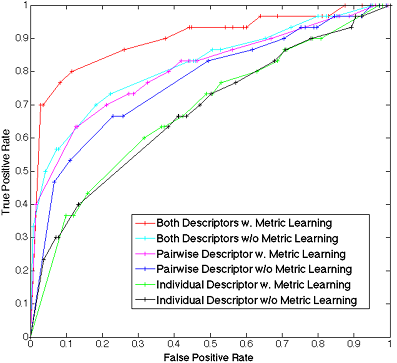
\includegraphics[width=2.4in]{ROC_s}
%\end{wrapfigure}

%%We have evaluated this approach using a subset of the Harvard Interactive Classroom Dataset, to be described in Section~\ref{sec:sys}, which is orders of magnitude larger than existing interaction benchmarks~\cite{UTdata,Choi:context,Choi:recogtrack}), in terms of the number of individuals (10-50 students per camera), the number of cameras (6), and the amount of time (more than 50 camera-hours). Through a combination of face detection and tracking, we obtained noisy tracks for all students in each camera and computed simple descriptors based on absolute and pair-wise relative head pose. With input from educational experts we manually identified the participants and start/end times of 112 distinct three-person discussions, and we separated these into four semantically-meaningful categories (e.g., three sitting in a row with two facing left vs. two in front and one behind). The annotated interactions range from a few seconds to tens of seconds in length, and detecting and recognizing them is a challenge because the number of by-standers is much larger than the number of participants ($M$ is between 10 and 20 while $N=3$), video quality is limited (low light, less than 15fps), and the visual cues for interaction are quite subtle. Detection results obtained using a leave-one-session-out evaluation scheme are shown in the ROC curves at right, with various parts of the system being isolated, leaving only individual $\mathbf{f}$ or pairwise $\mathbf{g}$ descriptors, and atomic distance matrices $\Sigma_{I}$, $\Sigma_{P}$ set to identity instead of being data-optimized as will be described in Section~\ref{sec:actlearn}. These results suggest that our preliminary system approach works well, and its performance and flexibility are further supported by tests showing that it provides state-of-the-art detection and recognition results on existing interaction datasets involving both humans~\cite{UTdata} and mice~\cite{CRIM13}, exceeding the accuracy in~\cite{UTdata} by 21\% and exceeding the accuracy in \cite{CRIM13} by 8\%.



%We have evaluated this approach using a subset of the Harvard Interactive Classroom Dataset, to be described in Section~\ref{sec:sys}, which is orders of magnitude larger than existing interaction benchmarks~\cite{UTdata,Choi:context,Choi:recogtrack}), in terms of the number of individuals (10-50 students per camera), the number of cameras (6), and the amount of time (more than 50 camera-hours). Through a combination of face detection and tracking, we obtained noisy tracks for all students in each camera and computed simple descriptors based on absolute and pair-wise relative head pose. With input from educational experts we annotated the participants and start/end times of 254 two-person and 112 three-person salient interactions separated into seven semantically-meaningful proxemes. The annotated interactions range from a few seconds to tens of seconds in length, and detecting and recognizing them is a challenge because the number of by-standers is much larger than the number of participants ($M$ is between 10 and 20 while $N=2,3$), video quality is limited (low light, less than 15fps), and the visual cues for interaction are subtle. Detailed results \cite{groupdet2013} suggest that our preliminary system works well on this data and also achieves state-of-the-art performances on benchmark datasets involving both humans~\cite{UTdata} and animals~\cite{CRIM13}.  


%While these early results are promising, they are only a small indication of what might be achieved. As part of the proposed activity, we will explore more sophisticated descriptor ensembles that allow, for example, larger cliques of relative descriptors and descriptors that are relative to the entire group. We will also explore measures of similarity that, instead of detection and recognition by matching, are well-suited for computing interaction saliency (i.e., interactions that are distinct from their space-time neighborhood) and for semi-supervised and unsupervised learning of categories (e.g., to automatically cluster the salient interactions discovered in a video collection).



%We will also explore spatio-temporal search algorithms that preserve the robustness to false detections and broken tracks brought by voting but are more efficient in time.



%%%%%%%%%%%%%%%%%%%%%%%%%%%%%%%%%%%%%%%%%%%%%%%%%%%%%%%%%%%%%%%%%%%%%%%%%%%%%%%%%%%%%%%%%%%%%%%


%\subsection{Salient Social Activities Discovery and Prediction}
%\label{sec:activity}
%
%The joint target recognition problem described in the previous section represent one scenario where social contexts significantly assist and improve a traditional computer vision task. In this section, we propose a \emph{new} computer vision task motivated and enabled by socialized metadata. This new task introduces new `words' that a picture or a video may convey, and the output conversely produces new clues for social sensing in related disciplines. 
%
%As the second major problem regarding socially-aware visual understanding, we propose to discover and predict salient social activities from videos, as well as still images if possible. The proposed task is novel from existing activity analysis and recognition work in three aspects: It seeks to discover salient social behaviors,  it  aims to predict activities using social contexts, and it directly builds upon realistic visual materials `in the wild'.
%
%\begin{figure}[t!]
%\begin{center}
%\includegraphics[width=\columnwidth]{socialbehavior}
%\end{center}
%\vspace{-0.25in} \caption{\captionsize 
%(a): Socially non-informative co-occurrence of articulations\cite{UTdata}; (b): Socially non-informative collective crowd activities\cite{Choi:context,Choi:recogtrack}; (c): Socially informative salient interactions; (d) Socially informative salient group interactions in the nature; (e) Socially meaningful three-way activity categories defined as `f-formations' by sociology\cite{Kendon1990}.\label{fig:socialbehavior}\afterfigspace}
%\end{figure}
%
%
%First, we propose to discover salient social activities. Specifically, social semantics assist in visual understanding in the way that they provide new social behavior categories for us to distill from images and videos, and these new social categories are informed by qualitative and quantitative sociology, which has been studying these behavior modes but never be automated by computer vision. As these new concepts are socially meaningful, they provide more expressive evidence about the social relationships among the individuals involved in the activities. We refer to these new social semantics as salient. In contrast to existing vision research, salient social activities are distinctive because they do not focus on non-informative interactions or group-wise behaviors. The non-informative interactions, for example, refer to the co-occurrences of two individual body articulations with limited clue about how the two individuals are related or exchange opinions, such as 'kick', 'punch', etc. (\cite{UTdata}, Fig. \ref{fig:socialbehavior}(a)). The non-informative group-wise behaviors, on the other hand, include collective activities of a crowd, within which there are no explicit interactions, such as 'group-walking', 'queueing', etc. (\cite{Choi:context,Choi:recogtrack}, \ref{fig:socialbehavior}(b)). Instead, the salient social activities are more  of gestural and conversational interactions, attention-response, as well as turn-taking meetings  (Fig \ref{fig:socialbehavior}(c)) where sociological semantics, as is interesting and important to the sociology research, can be derived. Fig. \ref{fig:socialbehavior} (e) shows diagrams for such socially meaningful activities categories, namely `f-formations', in three-way interactions that have been under the investigation of sociology. Moreover, we will develop generic salient socialized discovering models and approaches, so that they accommodate activities of social populations of animals and insects (Fig. \ref{fig:socialbehavior}(d)).
%
%Second, we propose to predict activities under social contexts. In this case, social semantics assist in visual understanding in the way that they serve as contextual information for restricting the more possible categories of activities that may occur between a specific group of individuals. This effort is also complementary to the usage of social contexts for identifying the targets presented in the previous section. Consider a simple illustrative example in which we would like to label a conversational scene in a movie as either a `negotiation� or a 'debate'. It is possible, in this case, that by the analysis of facial expressions, gestures, and poses, we still have difficulty in distinguishing the two. However, by appropriate face recognition in association with other metadata of the movie, probably with the help of social contexts as introduced in the previous section, we may gain solid confidence regarding the social relationship between the speakers as either `cooperative' or 'adverse'. A cooperative relationship are more likely to imply a negotiating activity, and an adverse relationship implies otherwise. A mechanism, similar to and in companion to the CRF formulation but adapted to video analysis, will be particularly useful.
%
%Third, we expect to develop approaches that directly take in realistic visual materials recording social activities of interest. On the one hand, realistic visual materials capture the social activities in unconstrained environment in the format of long-term surveillance videos of public areas with irrelevant human beings co-existing with socially engaged actors as well as scene/background clutter. Our approach will be one that can effectively and efficiently localize and retrieve salient social activities in space and time from these large volumes of cluttered image sequences. On the other hand, realistic visual materials such as surveillance videos and web videos are frequently in low and varying frame-rate, in low resolution, blurry, as well as in adverse view-points. Our effort will be handling all these realistic conditions and providing robust and practical tools that process more than those simulated, high-quality, manually pre-processed data \cite{UTdata,Choi:context,Choi:recogtrack}.
%
%\subsubsection{A prototype system and preliminary results}
%
%\begin{figure}[t!]
%\begin{center}
%\includegraphics[width=\columnwidth]{prototype}
%\end{center}
%\vspace{-0.25in} \caption{\captionsize 
%The prototype hardware and software infrastructure for analyzing socialized human behaviors in an indoor environment at Harvard University.\label{fig:prototype}\afterfigspace}
%\end{figure}
%
%As an initial attempt to analyze socialized human behaviors in an indoor environment, we have built up a prototype hardware and software infrastructure at Harvard University. As shown in Fig. \ref{fig:prototype}(a), the hardware part of the prototype system mainly consists of a networked audio-visual recording system for large-scale recording of student interactions in a Harvard College lecture hall. The system records audio and video from approximately one hundred students during each lecture in conjunction with the audience responses through an online teaching-learning application. The video system uses six IP cameras that together provide resolution that is high enough to achieve face-based identity recognition of each student in the audience. The audio system is an innovative design consisting 48 omnidirectional boundary microphones mounted inconspicuously among the seats, and outputting sound from each microphone recording to a single user-friendly mp3 audio file.To automatically analyze the videos, we have developed a robust computational suite of computer vision tools. This software consists of several fundamental modules that directly distill behavioral descriptions from raw videos, as well as a high-level module that detects salient social activities of interest from a new video and retrieves similar social activities. 
%
%
%With this established classroom observation system and these fundamental modules, we have successfully collected and processed a large-scale classroom behavior database consisting of 100 video clips in total. The students are seated in a regular lecture hall and are observed by a camera array with non-overlapping fields of view. The classroom is ``interactive'' because at various times throughout the lecture students are invited to engage in ad-hoc group discussions about problems provided by the instructor. The scale of our database is orders of magnitude larger than state-of-the-art computer vision datasets (e.g. those used in \cite{UTdata,Choi:context,Choi:recogtrack}), in the number of individuals (10-50 students per camera), the number of cameras (6), and the amount of time (100 minutes per camera, per recording, equaling over 3,000 minutes in total). Through a combination of face detection and tracking, we obtained noisy tracks for all students in each monocular video, upon which we developed descriptive modules that directly extract descriptiors such as head pose and body motion, we have also implemented a high-level module for behavior analysis based on similarity between two social groups, as depicted in Fig. \ref{fig:prototype}(b). In this module, the behavior of each individual is represented by a combination of the head pose and the motion of torso and arms (using the method of histogram of optical flows). The social behavior of a group is then represented by the configuration in space and time of the behaviors of its participants. With this social activity representation, the module detects a salient social activity from a new video and retrieves similar social activities from our established database. This functionality is illustrated in Fig. \ref{fig:prototype}(b), where our system has discovered a three-way conversation by identifying the participants of this conversation and the time span (several to tens of seconds) of this event. Based on the behavior representation for this space-time social interaction, the system searches the remainder of the database and retrieves a list of exemplars containing similar social behavior, ranked in the descending order of the similarities with the query. In this way, any manual annotations associated with the query video can be propagated to the top-ranking exemplars, and we are now taking this approach to propagate our manual annotations across the whole database. 
%
%
%\begin{figure}[t!]
%\begin{center}
%\includegraphics[width=\columnwidth]{dataset_compare}
%\end{center}
%\vspace{-0.25in} \caption{\captionsize 
%(a-1)-(a-3): Examples of the three categories for two-person interactions; (b-1)-(b-4): Examples of the four categories for three-person interactions; (c) Preliminary performance comparisons of our social activity retrieval software.\label{fig:dataset_compare}\afterfigspace}
%\end{figure}
%
%
%To evaluate the effectiveness of the social behavior retrieval module, we manually identified the participants and start/end times of all two-person, three-person, and four-person interactions, obtaining 254 two-person and 112 three-person interactions in total to constitute the entire database. In consultation with education experts we define interaction categories based on the geometric configurations of the participants: three categories for 2-person interactions (same row; different rows with left agent in front; different rows with right agent in front) and four categories for 3-person interactions. Example images for each category can be found in Fig. \ref{fig:dataset_compare}(a)(b). The annotated interactions range from a few seconds to tens of seconds in length. Since the raw videos arise from five different hour-long session, and we adopt a leave-one-session-out evaluation scheme in partitioning training samples (exemplars) from test samples (inputs). We study classification performance for 2-person and 3-person interactions, where we measure the accuracy of inferred interaction categories. Our low-level modules include both pose descriptors and relative motion descriptors, and our high-level module employs Metric Learning (ML). To evaluate the effectiveness of all these functionalities, we turned off some of components as baselines and compared with the full module with all components on. Fig. \ref{fig:dataset_compare}(c) shows the average true positive rates vs. false positives when classifying detected interactions into the three or four categories. As expected we see that performance improves when more parts of the system turned on, which implies that our prototype infrastructure has achieved reasonable technical quality.
%
%In our proposed research, we aim to enrich the descriptions of the social behaviors in the current prototype system, explore more accurate and robust comparison and retrieval mechanisms, and in particular, design novel modules for integrating social contextual annotations to allow our framework to be fully `socially-aware'.
% !TEX root = SocialVision2014.tex

%\subsubsection{Learning social interaction detectors and categories}
\subsection{Robust graph coarsening}
\label{sec:actlearn}
\vspace{-5pt}


\begin{figure}[t!]
\begin{center}
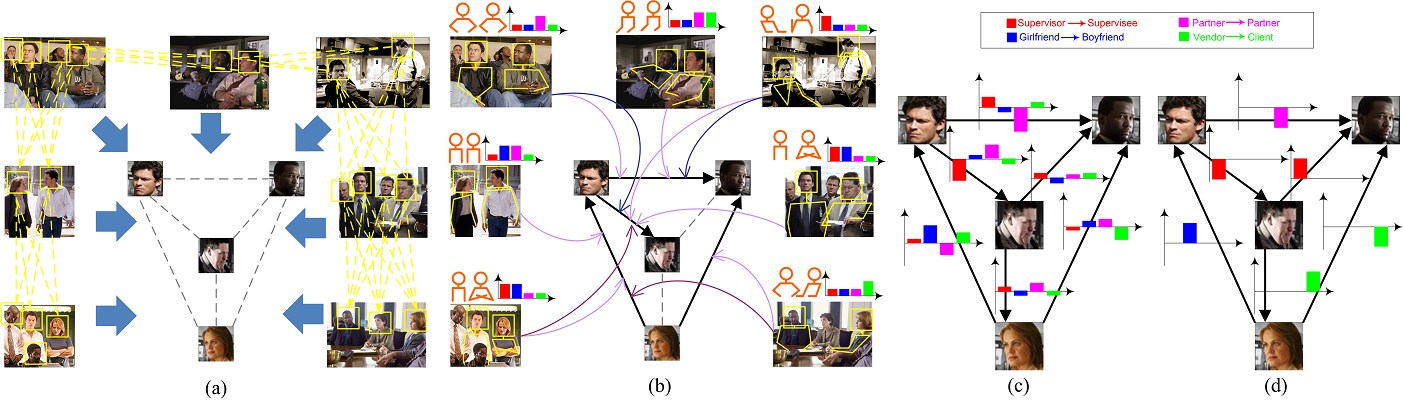
\includegraphics[width=\columnwidth]{SP_on_Graph}
\end{center}
\vspace{-0.25in} \caption{\captionsize 
Semantic image processing for detecting and classifying proxemes in image/video collections. (Details about the right box in Figure~\ref{fig:intro}) (a) Robust graph coarsening to identify the unique individuals (nodes) in the social graph; (b) transferring noisy relationship estimates from observed image targets to the graph edges; (c) Filtering on the graph edges to denies the multi-dimensional relationship signals and to complete the missing links; (d) Joint multi-way signal detection over all edges to determine the relationship types under higher-order constraints. \label{fig:SP_on_Graph}\afterfigspace}
\end{figure}

The computational representation of social interactions paves the way from images toward social relationships: By detecting and classifying instances of proxemes that occur between image targets, we may estimate the distribution over possible relationship types between each pair (triple, or higher order tuple) of targets, as long as the proxemes are informative about relationships. These socially-informative proxemes may be achieved by definitions and discoveries by social science experts, such as described in the previous section. However, experts are not available to exhaustively study every social setting. Instead, we require new unsupervised or semi-supervised data-driven methods that can learn socially-informative proxemes from unstructured image and video collections.

In the mean time, we require methods to obtain the nodes in the social graph � the unique individuals existing in the imagery collection � from the massive targets generated by face/human detection, as illustrated in Figure~\ref{fig:SP_on_Graph}(a). This is because individuals almost surely re-appear when repeatedly observed, and there are much more targets than unique individuals. 

Given a collections of interaction specimens from a social setting, the interaction representation provides a way to compute the similarity $S({\cal E},{\cal E}')$ between any two interaction specimens (in a massive specimen-specimen graph) that are characterized by descriptor ensembles $\cal E$ and ${\cal E}'$, and our goal is to distill another much smaller graph on which each node represents a socially-informative proxeme.  Given a collections of human targets from the same social setting, state-of-art tools such as �face verification� also provide a similarity between any two targets (in a massive target-target graph), and our goal is again to distill the much smaller social graph on which each node represents a unique individual. Both tasks that condense a big graph into a small one are referred to as graph coarsening. 

Despite that the problem setting seemingly resembles clustering (e.g. spectral clustering), where each original node is to be assigned to a node in the coarsened graph, there are several major challenges that distinguish the problem from conventional clustering tasks. First, face or human detections may produce false-detections on non-human targets, and the coarsening method must account for the outlier specimens consisting of these false detections. Second, only a tiny subset of space-time regions in video (and a small subset of pixels in an image) will constitute useful proxemes, and quite some �by-standers� that do not belong to the social graph of interest may sparsely appear in the imagery, so the algorithm must account for a coarsened graph of useful nodes (of meaningful proxemes or significant social members), in the existence of substantial �background clutter�. Third, the method must be able to effectively exploit spatio-temporal constraints among the targets: two targets co-occurring in the same scene must be affiliated to different coarsened nodes, and targets overlap in space over time are likely affiliated to the same nodes. Fourth, environmental information may induce implications about higher-order grouping effects: tuples of targets that frequently co-occur in the same type social scene (e.g. office space), which may be computed by semantic scene classification, and those that frequently co-occur in a different type of social scene (e.g., night club), are more possibly affiliated to different sets of coarsened nodes. The coarsening method is expected to make use of these contextual information as well. Finally, in case that expert knowledge is limitedly infused, the method must exploit these weak supervision and therefore accommodate weakly-supervised working mode.

During the award period, we will explore new classes of graph coarsening mechanisms to address these challenges in a unified manner. For the last challenge, we will leverage the PI�s expertise on �domain adaptation�, a strategy in handling weak supervision, and build upon frameworks for domain adaptation that have been recently introduced for recognizing object and single-agent actions by the PIs and others~\cite{LiZickler2012,Li2011}. For the first and second challenges, we will explore techniques that build upon our representation of interaction similarity (\ref{subsec:activity} and  \cite{groupdet2013}) to merge salient nodes while simultaneously refining the parameters of the similarity model itself. Figure 3 provides a hint at the potential utility of these research directions. This figure shows the results, on both a video corpus and an image corpus, of a simple baseline system for discovering proxeme categories without supervision. In this baseline system, we iterate between: 1) merge nodes by affinity propagation~\cite{frey07affinitypropagation} using the similarity score $S({\cal E},{\cal E}')$ of Sec.\ref{subsec:activity}; and 2) updating the �atomic� metrics $I$ and $P$ that control that similarity score. In companion, we will also explore establishing non-parametric Bayesian models, such as Dirichlet Process Gaussian Mixture Models(DP-GMM), in the space of spectral embedding of the nodes, because DP-GMM will allow flexible number of clusters (coarsened nodes) as well as a long-tail cluster which specifically accounts for the �background clutter�. In accordance with these explorations, we will borrow from such as constrained-EM algorithm, so that mechanisms to address the third and fourth challenges will be seamless integrated.


Figure~\ref{fig:prodic}(a) shows representative frames from dynamic proxemes discovered in a subset of the Harvard Interactive Classroom Dataset (See~\ref{sec:sys}) using individual and pairwise descriptors $\mathbf{f}, \mathbf{g}$ based on histograms-of-flow. Each column is a proxeme, and it is visualized using a representative frame from each of three different exemplars of that proxeme. Upon examination, we see the emergence of four interactive gesturing patterns in a classroom environment: dominant vigorous gesturing on the left or right; mild, simultaneous gesturing by both; and simultaneous engagement with an object. Figure~\ref{fig:prodic}(b) contains results of applying the same process to an unstructured photo collection using individual and pairwise descriptors $\mathbf{f}, \mathbf{g}$ derived from crowd-sourced image coordinates of body key-points. Again, each column is a proxeme, and the figure shows four exemplars for each proxeme. Even though these proxemes are discovered without any social side information, we notice substantial correlation between these proxemes and parent-child relationships, romantic partner relationships, and relationships between siblings or friends. These promising early results inspire us to systematically explore robust graph coarsening paradigms to learn environment- specific proxemes, and to distill social nodes from image targets, in a systematic manner and on a much larger scale. 
%\subsubsection{Learning an environment-specific dictionary of proxemes}

%Given a set of pre-defined proxemes, we can detect and recognize instances of these categories using the methods of the previous section. But how do we obtain these proxemes in the first place? As discussed in the related work, some of these categories can be manually discovered and defined by social science experts, but experts are not available to exhaustively study every setting.\comment{, we certainly cannot limit ourselves to those.} Instead, we require new unsupervised and semi-supervised methods that can learn socially-informative proxemes from unstructured image and video collections.

%There are two major challenges in learning socially-informative proxemes that distinguishes the problem from regular clustering tasks. First, only a tiny subset of space-time regions in video (and a small subset of pixels in an image) will constitute useful proxemes, so the learning algorithm must be able to automatically identify the useful intervals within substantial ``background clutter". Second, the algorithm must be able to effectively exploit side information whenever it is available, including textual metadata and relationship information from non-visual sources. 

%we do not  However, to obtain these categories in another specific domain, another group of domain experts and extensive manual annotations are required, which has been the practice in social science in obtaining proxemes (e.g., those shown in Fig. \ref{fig:socialbehavior} (c)(d)). This requires tremendous amount of manual efforts that can be sometimes prohibitive, and the obtained proxemes do not automatically generalize to other domains. In some domains, there may not be experts or knowledge available \emph{a priori}, and commonly studied interactions categories \cite{UTdata} may not be informative: `kicking' and `punching'  are rare in reality, `hand-shaking' does not occur frequently between those with close relations, and `hugging' is too common to distinguish family relationship from professional peers.


\begin{figure}[t!]
\begin{center}
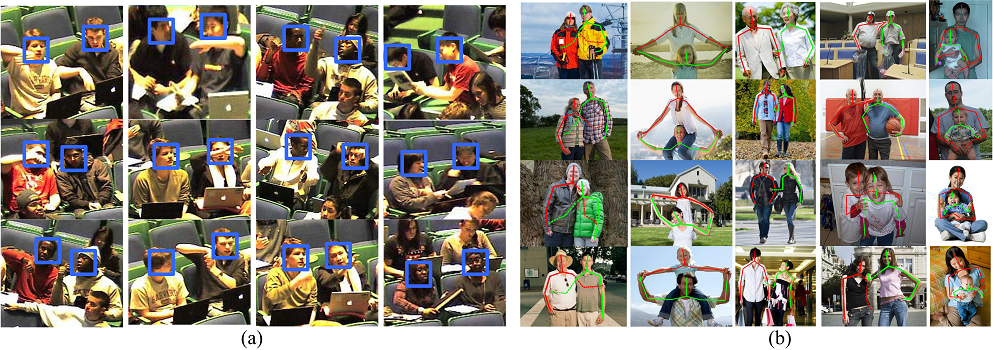
\includegraphics[width=\columnwidth]{socialdic}
\end{center}
\vspace{-0.25in} \caption{\captionsize (a) Dictionary of proxemes of pairwise gesturing unsupervised learned from the Harvard Interactive Classroom Dataset. (b) Socially-informative dictionary of proxemes of pairwise poses unsupervised learned in Flickr photos. Each column represents a proxeme.}
\label{fig:prodic}\afterfigspace
\end{figure}

%\begin{wrapfigure}{r}{0.4\textwidth}
%\vspace{-20pt}
%  \begin{center}
%    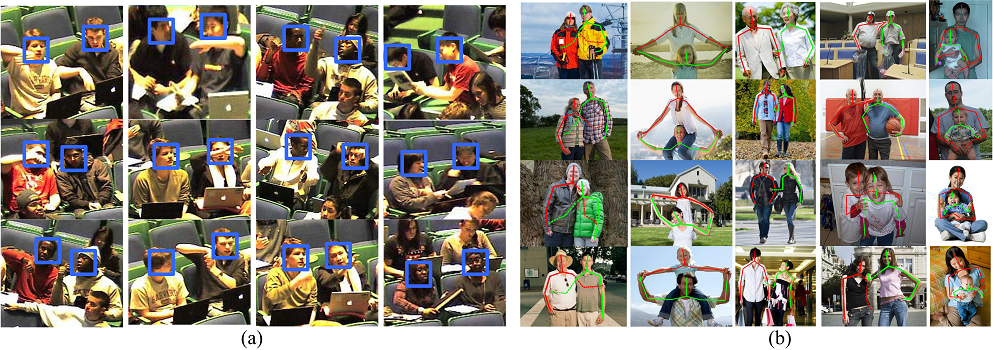
\includegraphics[width=0.4\textwidth]{socialdic}
%  \end{center}
%  \vspace{-20pt}
%   \caption{ Socially-informative dictionary of proxemes of pairwise poses. Each column represents a proxeme.}
%   \vspace{-15pt}
%\label{fig:flicker}
%\end{wrapfigure}

%During the award period, we will explore a variety of techniques to deal with these challenges. For the second challenge, we will treat side-information as interaction signals from other, non-visual ``domains'', and we will build upon frameworks for domain adaptation that have been recently introduced for recognizing object and single-agent actions by the PIs~\cite{LiZickler2012,Li2011} and others. For the first challenge, we will explore techniques that build upon our preliminary model for interaction similarity (Sec.~\ref{subsec:activity} and \cite{groupdet2013}) to develop techniques that cluster salient samples based on the similarity while simultaneously refining the parameters of the similarity model itself. Figure~\ref{fig:prodic} provides a hint at the potential utility of these research directions. This figure shows the results, on both a video corpus and an image corpus, of a simple baseline system for discovering proxeme categories without side information. In this baseline system, we iterate between: 1) clustering samples by affinity propagation~\cite{frey07affinitypropagation} using the similarity score $S({\cal E},{\cal E}')$ of Sec.~\ref{subsec:activity}; and 2) updating the ``atomic'' metrics $\Sigma_{I}$ and $\Sigma_{P}$ that control that similarity score.

%Figure~\ref{fig:prodic}(a) shows representative frames from dynamic proxemes discovered in a subset of the Harvard Interactive Classroom Dataset using individual and pairwise descriptors $\mathbf{f},\mathbf{g}$ based on histograms-of-flow. Each column is a proxeme, and it is visualized using a representative frame from each of three different exemplars of that proxeme. Upon examination, we see the emergence of four  interactive gesturing patterns in a classroom environment: dominant vigorous gesturing on the left or right; mild, simultaneous gesturing by both; and simultaneous engagement with an object. Figure~\ref{fig:prodic}(b) contains results of applying the same process to an unstructured photo collection using individual and pairwise descriptors $\mathbf{f},\mathbf{g}$ derived from crowd-sourced image coordinates of body key-points. Again, each column is a proxeme, and the figure shows four exemplars for each proxeme. Even though these proxemes are discovered without any social side information, we notice substantial correlation between these proxemes and parent-child relationships, romantic partner relationships, and relationships between siblings or friends. 

%Inspired by these promising early results, we will systematically explore the learning of environment-specific proxemes on a much larger scale. This includes formalizing the objective functions that are being optimized by iterative techniques like our baseline, and understanding how to incorporate side-information into this process. This research will allow the automatic creation of environment-specific proxeme dictionaries that are analogous to dictionaries of textons~\cite{leung2001representing} or visual words~\cite{grauman2005pyramid,lazebnik2006beyond}, and that serve as a bridge between imagery and social networks.




%\subsubsection{From target graph to social graph}


%%%%%%%%%%%%%%%%%%%%%%%%%%%%%%%%%%%%%%%%%%%%%%%%%%%%%%%%%

%\subsubsection{Associating identities with image targets}
%\label{sec:assoc}

%\boldstart{Associating identities with image targets}. To infer a social network from descriptors extracted from detected and tracked agents, we must first associate these vision-based descriptors with the identities of the tracked agents. While face recognition and identity recognition have progressed tremendously during the past decade (see Section~\ref{sec:background}), these systems will continue to suffer from uncertainty well into the future, especially when the input images and videos are low in quality. A key challenge we will address, therefore, is how to succeed in spite of this uncertainty. In doing so we will depart from the implicit assumptions in most existing approaches in network reconstruction, where even though additive or multiplicative noise might exist in the measured social affinities, these measurements are properly associated with the correct identities/nodes.

%\boldstart{Associating identities with image targets}. To infer a social network for detected and tracked targets, we must first associate these targets with their identities, and we assumed that the association is perfect in the discussion about network estimation. While face recognition and identity recognition indeed have progressed tremendously (see Section~\ref{sec:background}), these systems will continue to suffer from uncertainty, especially when the input images and videos are low in quality. A key challenge we will address, therefore, is how to succeed in spite of this uncertainty, a challenge that is rare in traditional social network analysis.

%In doing so we will depart from the implicit assumptions in most existing approaches in traditional social network analysis, where even though additive or multiplicative noise might exist in the measured social affinities, these measurements are properly associated with the correct identities/nodes.

%One simple approach we will explore is as follows. Suppose we have detected and tracked $L$, and that a face recognition system outputs for each a $K$-dimensional probability histogram $h_l(k)$ describing the likelihood of target $l$ being identity $k$. If facial recognition were perfect, each pair of tracks would be used to produce one set of visual cues $\vy^u(i,j)$ linked the (certain) identities $i$ and $j$. In the presence of uncertainty, we can enumerate all possible $\prod_{l=0}^{L-1}(K-l)$ assignments, and then (conceptually) duplicate the video $\prod_{l=0}^{L-1}(K-l)$ times considering in each copy that the $L$ targets are assigned according to one of the possible assignments $\{k_1, k_2, \cdots, k_L\}, k_l\in\{1,2, \cdots, K\}$. This produces multiple outputs from each visual source---a descriptor of the form $\vy^u(k_i,k_j)$ for each of the $\prod_{l=0}^{L-1}(K-l)$ conceptual copies.

%The advantage of this approach is that it allows aggregating all of the information available from the recognition system, which we do by ``pooling'' the visual descriptors from all $\prod_{l=0}^{L-1}(K-l)$ copies. We will consider maximum-pooling approaches, $k_l^{*}=\max_{k}h_l(k)$, that select the most probable identity for target $l$ and use only the maximum assignment $\{k_1^{*}, k_2^{*}, \cdots, k_L^{*}\}$ to compute the social cues $\vy^u$ associated with identities $\{k_1^{*}, k_2^{*}, \cdots, k_L^{*}\}$. This strategy essentially assigns each target to a single (possibly incorrect) identity. We will also consider weighted average pooling, where every video copy corresponding to assignment $\{k_1, k_2, \cdots, k_L\}$ contributes to the social cues $\vy^u$ but with a confidence score proportional to the confidence of the recognition system, e.g., $\prod_{l=1}^{L}h_l(k_l)$. In this research, we will not just pursue good empirical results: We will also pursue tractable statistical models for identity uncertainty that can be characterized rigorously, with the goal of creating knowledge that can be more broadly applied to statistical signal processing on graphs and other relational data structures.


%Given a set of defined interaction categories, we can detect and recognize instances of these categories using the methods of the previous section. But how do we learn the categories in the first place? How can we make use of labeled samples of interactions? What if few labeled samples are present? In this subsection, we show preliminary results of using category-labeled interaction training samples to maximize the performance of detection and recognition described above, and we describe our plans for exploring semi-supervised and unsupervised learning.

%The detection and recognition system of Section~\ref{subsec:activity} incorporates learnable metrics $\Sigma_I$, $\Sigma_P$ for measuring ``atomic'' distances between descriptors in Eq.~\ref{eq:partial-matching}. These metrics can be optimized to improve detection by better discriminating between interactions and background, and when exemplars are labeled by category, they an be optimized to improve recognition by better discriminating between interaction categories. In our early experiments, we have shown that both of these can be accomplished simultaneously using an adaptation of the Large Margin Nearest Neighbor (LMNN) framework~\cite{Weinberger:ML}, and this is the procedure used to generate the ``w/ Metric Learning'' results in the previous section. It is one simple example of how annotations can be used to learn effective models for interaction categories, thereby allowing a single computational framework for interaction analysis to succeed in a wide variety of environments.

%We do this by constructing two collections from our database exemplars. The collection $\mathcal{P}$ contains all pairs of instantaneous interaction ensembles that are of the same category and occur roughly in the same temporal location within the interaction instances, together with their ``ground-truth" matchings. The collection $\mathcal{M}$, on the other hand, is comprised of ordered triples $(h,k,l)$ in which ensemble $h$ is the same category as ensemble $k$ and ensemble $l$ is either of a different category or background. Having defined these two collections, the Mahalanobis parameters are found by solving
%\begin{equation}
%\label{classify}
%\begin{split}
%&\min_{\Sigma_{I}, \Sigma_{P}} \sum_{(u,v)\in\mathcal{P}}\hat{D}(\mathcal{D}_{u}, \mathcal{D}_{v}, W_{u,v})+\gamma\sum_{(h,k,l)\in\mathcal{M}}\xi_{h,k,l},\\
%&\textup{s.t.}  \hat{D}(\mathcal{D}_{h}, \mathcal{D}_{l}, W)-\hat{D}(\mathcal{D}_{h}, \mathcal{D}_{k}, W_{h,k})\ge 2-\xi_{h,k,l}, \Sigma_{I}\succeq 0, \Sigma_{P}\succeq 0, \xi_{h,k,l}\ge0,
%\end{split}
%\end{equation}
%where $W_{u,v}$ is the ``ground-truth" matching for pair $(u,v)$ and $W$ is an arbitrary matching. The minimization over either $\Sigma_{I}$ or $\Sigma_{P}$ is exactly a Large Margin Nearest Neighbor (LMNN) problem \cite{Weinberger:ML}, and we apply LMNN multiple times to separately learn one distinct pair of ($\Sigma_{I}, \Sigma_{P}$) for each value of the number of interaction participants. 

%One of our goals in the proposed activity is to develop tools that allow effective learning of models for interaction categories with many fewer labeled samples. This is motivated by immense manual effort required to obtain these samples. We will explore semi-supervised and unsupervised methods for discovering interaction categories in video collections, based on measures of interaction saliency and between-ensemble similarity measures that incorporate loose space-time structural constraints. We will also explore the use of side information, which might comes in the form of textual metadata or relationship information drawn from non-visual sources. This side-information can be regarded as interaction signals from another ``domain'', and consequently might be exploited in a domain adaptation framework like those recently developed by the PIs~\cite{LiZickler2012,Li2011}. 






% !TEX root = SocialVision2014.tex

\subsection{Network Reconstruction: Multi-Dimensional Signal Processing on Edges}
\label{sec:vis2net}
\vspace{-5pt}

Let $i$ and $j$ be two nodes representing two nodes, and let $y_{ij}(k)$ to be the probability of the $k$-th type of directional relationship $i\rightarrow j$ that takes a value between $-1$ and $+1$. We allow �negative probability� to encode the directional property of social relationships: If the $k$-th type of relationship, for example, refers to �parent$\rightarrow$child�, then $y_{ij}(k)=0.3$ means that individual $i$ is the parent of individual $j$ with probability 0.3, and  $y_{ij}(k)=-0.7$ means that individual $i$ is the child of individual $j$ with probability 0.7.  (Undirectional relationship types may be treated as directional where the sign does not matter.) This probability defined on every edge of the social graph may be computed from that defined on the target pairs, because the graph coarsening procedure associates a probability $p_{mi}$, for a particular target $m$ to be condensed in the social node $i$: As a result, given the probability $z_{mn}(k)$ of the $k$-th type of directional relationship between targets $m$ and $n$ computed from the proxeme between them, it is straightforward that $y_{ij}(k)=\int_{mn}p_{mi}p_{nj}z_{mn}(k)dmdn$, as illustrated in Figure~\ref{fig:SP_on_Graph}(b). Note that the semantic image processing tools also provide other individual attributes such as age and gender~\cite{Gender, Age} to the pair $(m,n)$, and the probability of a particular type of relationship, in analogy to $z_{mn}(k)$ but induced by these personal attributes,  may also be computed and transferred to edge $(i,j)$ in a similar manner. 

With these quantities $y_{ij}(k)$ computed, our goal is to compute a set of social adjacency matrices $A(k), k=1,2,�,K$, each of size $N\times N$, where $K$ is the total types of relationships under considerations, $N$ is the number of social members. Each element $A_{ij}(k)$ takes one of the three discrete values -1, 0, or 1, and by definition of the directional relationship, each adjacency matrix is skew-symmetric $A(k)=-A(k)^T$. This requires three-way signal $A_{ij}(k)$ detection over edges of the social graph using �observation� $y_{ij}(k)$.

A set of challenges distinguishes the problem from the majority of conventional studies on signal processing on graphs. First, we require to detect discrete signals defined on edges (1-cells) and this is equivalent to operating in the space of 1-cochains. This differs from the focus of the current studies on graph signal processing or machine learning, which operate on the continuous real or complex signals defined on nodes (0-cochains). Second, the observations $y_{ij}(k)$ are noisy, not only because of imperfect detection and classification or cumulative computing errors, but more significantly because that any two individuals do not necessarily co-occur or interact frequently enough to give rise to adequate proxemes: For some edges, these ``observations" will be unreliable or completely missing. \comment{if few proxemes may be extracted between nodes $i$ and $j$, and it may be even completely missing if no proxeme is available.} Third and finally, the signals across different types of relationships are structurally constrained, just as shown by social network research, where social networks are found to include multiple overlapping and structural communities: Consider the example where the $k_1$-th, $k_2$-th, and $k_3$-th types of relationships refer to �mother$\rightarrow$child�, �wife$\rightarrow$husband�, and �farther$\rightarrow$child� respectively, and the hypothesis pair $A_{ij}(k_1)=1$ and $A_{il}(k_2)=1$ requires the hypothesis for the 1-cochain $(j,l)$ to be $A_{jl}(k_3)=-1$. Therefore, signals must be collaboratively detected over 1-cells respecting the semantic relationship constraints across the relationship types over higher-order cells. 

To address these challenges, we will develop generic frameworks for collaborative detection of multiple discrete signals defined on edges under unreliable and missing observations\comment{ across multiple relationship types, which are mutually regularized by structural relationship constraints among these types}.  To begin with, we will explore a 2-step approach. In the first step, we will design edge-wise energy minimization models (EEMM) for filtering (denoising) the unreliable directional relationship probability signals of each type and for completing the missing signals over the missing edges. In the second step, we will apply prime-dual transformation to convert structural constraints among subset of 1-cells to independent unary constraints over the 0-cells in the dual cell complex, and this enables us to develop analogies to discrete random-field optimization to solve the discrete decision problem in the dual complex representation.

\boldstart{(1)} We will first develop EEMM for filtering the edge-wise directional probabilities $y_{ij}(k)$ supported by observed salient proxemes to obtain `cleaner� probabilities $\hat y_{ij}(k)$ over all edges, including those missing co-occurrences in the imagery, as illustrated in Fiure~\ref{fig:SP_on_Graph}(c). The optimal clean signals must satisfy two criteria: First, it must respect the observed signals over the edges supported by observed salient proxemes, preserving `data fidelity�. Second, it must behave as a `low-pass� filter to preserve the smooth components in the observed signal, treating the `high-frequency� component as noise incurred for various reasons. As a result, the EEMM minimizes a combination of data fidelity and smoothness
\begin{equation}
\min_{\hat{\mathbf{y}}(k)}\hat{\mathbf{y}}(k)^{T}L_e\hat{\mathbf{y}}(k)+\gamma\sum_{(i,j): y_{ij}(k)~\textup{exists}}\|y_{ij}(k)-\hat y_{ij}(k)\|^2
\end{equation}
where $L_e$ represents the edge Laplacian. It has been proved the edge Laplacian can be rewritten as $L_e=N_{1}N^{*}_{1}+N^{*}_{2}N_{2}$ where $N_{1},N_{2}$ and $N^{*}_{1}, N^{*}_{2}$ are called the boundary operators and co-boundary operators \cite{Grady10}. 

Now that the problem has been transformed to a filter design problem � to determine the boundary operators and co-boundary operators. we may further employ the facts that decompositions $N_{1}N^{*}_{1}=PG_{0}P^{T}G^{-1}_{1}$ and $N_{2}N^{*}_{2}=G_{1}Q^{T}G^{-1}_{2}Q$ exist \cite{SpectralChung,Grady10}, where $P$ and $Q$ are the node-edge, edge-face (2-cell) incidence matrices respectively, and consequently further transform the filter design problem to determine the diagonal metric tensors $G_0$, $G_1$ and $G_2$. As the diagonal element $g_e(i,i)$ encode the �weight�� assigned to the i-th e-cell, one possibility to specifying these weights, is simply to take $G_1=I, G_2=I$, and let $g_0(i,i)$ to be the `weight' on the i-th node as $g_{0}(i,i)=\sum_{j}s(i,j)$ , where $s(i,j)$ are pairwise similarities computed from facial similarities, age/gender attributes, scene types, occurrences, and other kinds of visual clues that may imply the social-affinity between two individuals. In the proposed research, we will explore other ways in accomplishing this filter design, we will also look into different algorithms in performing the optimization, by deriving a corresponding quadratic programming algorithm, or adapting from the backward Euler method \cite{Press:2007}.

\boldstart{(2)} With filtered directional relationship probabilities\comment{ for all individual pairs and all relationship types}, we will in the second step design collaborative detection of multiple discrete signals defined on edges across multiple relationship types regularized by structural relationship constraints, as illustrated by Figure~\ref{fig:SP_on_Graph}(d).  To this end, we may harness Poincare duality property\comment{ for calculus defined on general cell complexes} \cite{SpectralChung,Grady10}, and transform each social graph, considered as a 2-complex, into its dual form. In the dual form, each 2-cell (face) in the primal complex consisting of three individuals becomes a 0-cell (node) in the dual, and the triple-wise structural constraints among the primal nodes are converted to constraints on this single node in the dual. The duality properties between the two forms also provides ways to compute the topologies of the dual complex in terms of the dual boundary operator and dual co-boundary operator, by which one may further derive the Laplacian for the dual complex\cite{SpectralChung,Grady10}.

This dual transformation leads a framework of labeling the dual nodes (i.e., the edge triples in the primal) as one of the triple-wise relationships, each of which is defined by three pairwise relationships. Given a dictionary of all possible triple-wise relationships, labeling a dual node into one of the triple-wise relationships is analogous to encoding it as a \emph{sparse} linear combination of all possible triple-wise relationships in the dictionary, while maintaining consistency between neighboring dual nodes (i.e., primal node triples with overlapping edges). Inspirations may be then drawn from such as sparse coding of image patches while maintaining consistency between overlapping patches \cite{EladPatchDictionary,ZoranSparsepatch}: We will develop sparse coding for labels of cell complexes, apply them to the dual nodes of the social graph, and transform the results back to the primal complex before obtaining the final relationship signal on every edge of the entire social graph.

Based on the findings during the exploration of the 2-step approach, we will continue to look into ways in unifying denoising, edge-completion, and signal detection. The unification will lead to optimization problems that are NP-hard, and we will leverage the expertise of PI Li, who has a history of formulating and solving optimization problems on non-traditional domains \cite{LiPAMI2012}. We will also generalize the approach to signals existing on higher-order cells by directly extending the discussions to higher-order Laplacian, filter design, and primal-dual transformations, and this will provide us the foundation to study larger-size community-wise signals. Last but not least, we will explore ways to scale up the model to accommodate massive number of social members, and we expect to explore frameworks in the spirit of a consensus of distributed local optimizers by PI Zickler and others \cite{ChakrabartiXGZ14}.

\subsection{Closing the Loop: Joint Image Processing and Graph Signal Processing}
\label{sec:closeloop}
\vspace{-5pt}
A longer term goal of our research is to allow synergistic collaboration between semantic image processing/recognition and social signal detection. We have argued that semantic image processing provides information about an underlying social network, but the converse is also true. As shown by PI Zickler and others~\cite{Stone2008,Stone2010}, social network information can serve as context to improve image-based recognition. We envision a future in which these two processes work together. When uncertainty in an image recognition system leads to low confidence output, the uncertainty propagates to the extracted social cues and therefore to the inferred social network graph. However, by reconstructing and denoising the graph as proposed above, we can improve our estimate of the underlying social network, and then carry this information back to the image data, use the the improved social network as context to correct errors and improve recognition models.




%This dual transformation establishes a random-field model for the dual complex, for which only unary and binary potentials are involved. As a result, discrete optimization procedures, either based on sampling or using linear programming approximation, may be derived for inferring in the dual complex. 


%\subsubsection{Filtering on the edges: relationship propagation incompletely observed  co-occurrence}

%\subsubsection{Detection relationship signals with higher-order relational constraints}

%In addition to analyzing social interactions in videos, we will investigate tools for analyzing social \emph{relationships}, in terms of the social network that embeds the people observed in an image and video collection. As is customary, we consider the social network of $K$ individuals to be an undirected weighted graph $G$, with $K$ nodes and a non-negative weight ($\in [0,1]$) on the edge between each node-pair. Each weight represents the social proximity, or strength of tie, between two people, and the weights are collected in a positive symmetric affinity matrix $A$ of size $K\times K$. As described in Sections~\ref{sec:intro} \& \ref{sec:background}, our goal is to develop network reconstruction methods that are well-suited for vision by simultaneously: 1) modeling the multiple-community structure of social networks; 2) incorporating a variety of noisy sources (i.e., social cues automatically extracted from images and videos of varying quality); and 3) tolerating identity errors and high levels of missing data.

%From detecting, recognizing, and counting occurrences of social proxemes, we will proceed to analyze \emph{social relationships}. As is customary, we consider the social network of $K$ individuals to be an undirected, weighted graph $G$, with $K$ nodes and a non-negative weight ($\in \{0,1\}$) on the edge between each node-pair. Each weight represents the social tie between two people, and the weights are summarized by a positive symmetric affinity matrix $A$ of size $K\times K$. As described previously, our goal is to develop network reconstruction methods that are well-suited for vision by simultaneously: 1) modeling the multiple-community structure of social networks; 2) incorporating noisy proxeme counts from a variety of noisy visual cues; and 3) tolerating uncertain identities and missing links.

%It has commonly been observed that social networks include multiple overlapping communities (e.g.,~\cite{AiroldiBFX08,Kim12}). Computationally, this means that the social distance between nodes is not scalar-valued but depends on the type of roles or memberships being considered (e.g.,~friends vs.~colleagues vs.~family). We refer to these types as different \emph{views} and we represent them by defining $G\triangleq\{A^{(v)}\}_{v=1}^{V}$, where $A^{(v)}$ is the affinity matrix summarizing the ties between every pair of nodes in the $v$th view. For example, if $v\in\{1,2,3\}$ corresponds to friends, family, and workmates, $A^{(1)}(i,j)=1$, $A^{(2)}(i,j)=1$, and $A^{(3)}(i,j)=0$ indicates that Alice ($i$) and Bob ($j$) are not biologically related but are simultaneously close friends and colleagues.

%The multiple views overlap in general, and the effective tie between each node pair depends on which view is be used to assess their relationship.

%In addition to considering multiple views, we will also account for social information coming from multiple distinct cues extracted from visual data, without these cues being associated with peoples' identities with complete certainty. To do this, we consider $S$ \emph{sources} producing socially-informative cues $\vy^s, s=1,2,\cdots,S$, with each $\vy^s(i,j)$ being a multi-dimensional descriptor computed from a distinct socially-informative visual cue related to person $i$ and person $j$. As an example, for a detected, tracked and correctly-identified pair of individuals Alice $(i)$ and Bob $(j)$, a set of sources could include (time-varying in videos): relative positions of the two detections $\vy^1(i,j)$ (or $\vy^1$ for short); relative head poses $\vy^2$; relative body poses $\vy^3$; distribution over interaction categories $\vy^4$ detected and recognized as in Section~\ref{sec:activity}; and scene category $\vy^5$. These cues will not generally be associated uniquely with one pair of individuals because of uncertainties inherent to face recognition and other forms of identity recognition, and this means that each source will generally produce from the same image or video sequence multiple differently-weighted outputs. For example, if we cannot visually distinguish Bob ($j$) from Charlie ($k$) then each source will produce from one video sequence two outputs that satisfy $\vy^s(i,j)=\vy^s(i,k)$.

%Out goal is to infer the set of affinity matrices $\{A^{(v)}\}$ from imagery, using proxeme counts and other visual descriptors as input. In general, there will be multiple proxeme dictionaries that are relevant to the same social network. For example, there may be one based on histograms-of-flow in surveillance videos, another based on head and body pose in higher-fidelity videos, and yet another based on relative body positions in photographs of the same individuals. We index by $u=1,2,\ldots,U$ the available proxeme dictionaries corresponding to different visual cues $u$, and we denote these proxeme dictionaries by $\mathcal{D}^{(u)}$. To robustly exploit the correlations between relationships and noisy proxeme counts,
%consider $S$ types of \emph{cues} yielding socially-informative proxemes $y^s\in\mathcal{D}^{(s)}, s=1,2,\cdots,S$, where $\mathcal{D}^{(s)}$ denotes the dictionary of the $s$th type of proxemes learned from the $s$th type of visual cue. As an example, a set of four types ($S=4$) of cues could include 1) relative positions of the two detections, 2) relative head poses (as used in the classroom videos), 3) relative body poses (as used in the internet images), and 4) short-term interactive actions characterized by flows.
%On the one side, each type of proxeme will not necessarily uniquely correspond to one type of social relationship. On the other side, despite that we learn the proxemes using manual annotations, at runtime we will use existing imperfect tools to compute the visual cue ( \emph{e.g.} \cite{poselet,pose_part} for pose estimation) before classifying it into one of the proxemes, and therefore the recognized proxeme may be erroneous. As a result of both uncertainties, for a detected, tracked and correctly-identified pair of individuals Alice $(i)$ and Bob $(j)$,
%we can learn from training data representations of $P(A^{(v)}(i,j) \mid y^u)$: the probability of a relationship between $i$ and $j$ according to the $v$th relationship view given a detected instance of a proxeme from the $u$th dictionary. An interesting challenge we must address is that identities $i$ and $j$ will also be noisy, since they will be inferred from face recognition and other biometric cues. For example, if we cannot visually distinguish Bob ($j$) from Charlie ($k$) then a single cue $u$ can produce two separate probabilistic signals: $P(A^{(v)}(i,j) \mid y^u)=P(A^{(v)}(i,k) \mid y^u)$.


%\boldstart{Multi-view network regression}. One of our project goals is to establish a unified, data-driven framework for reconstructing multi-view network representations (affinity matrices $A^{(v)}$) from multiple noisy, heterogeneous visual sources. We refer to this problem as multi-source multi-view network estimation, and we will address it using an architecture comprised of $V$ trained \emph{oracles} $\Psi_{v}$ that each provide an estimate of one view $\hat{A}^{(v)}$ from all available vision-based descriptors $\bar{\vy}=[\vy^1,\vy^2, \cdots,\vy^S]$. That is, $\hat{A}^{(v)}=\Psi_{v}(\bar{\vy})$, with $\Psi_{v}$ learned from data according to the following general approach. Given collections of vision-based social cues $\{\bar{\vy}_{n}\}_{n=1}^{N}$ attributed to $N$ different unknown social network graphs, optionally supplemented by additional collections $\{\bar{\vy}_{n}\}_{n=1}^{M}$ attributed to $M$ graphs that are known (i.e., known
%affinity matrices $\{\bar{A}^{(v)}_{m}\}_{m=1}^{M}$, perhaps through non-visual metadata like that described in Section \ref{sec:sys}), we will investigate a family of objectives of the form
%\begin{equation}\label{eq:sensing}
%\{\Psi^{*}_{v}\}=\arg\!\!\!\!\!\!\!\!\min_{\{\Psi_{v}\},\{\hat{A}^{(v)}_l\}_{l=1}^{N+M}}\sum_{m=1}^{M}\mathcal{J}\left(\{\Psi_{v}\}, \{\bar{\vy}_m\}, \{\bar{A}^{(v)}_m\}\right)+\tau\left(\{\hat{A}^{(v)}_m\},\{\hat{A}^{(v)}_n\}\right)+\gamma\left(\{\Psi_{v}\}\right).
% \end{equation}
%The first term $\mathcal{J}$ in this expression is a loss term that gives preference to oracles that agree with the $M$ known graphs. For example, $\mathcal{J}(\{\Psi_{v}\}, \{\bar{\vy}_m\}, \{\bar{A}^{(v)}_m\})=\sum_{v=1}^{V}\|\Psi_{v}(\vy_m)-A^{(v)}_m\|^{2}$ would measure discrepancy from the known graphs in a least-square sense. To prevent over-fitting, the complexity of the oracles is restricted by a regularization term $\gamma()$, whose form depends on the choice of oracles, such as Gaussian process regression \cite{GPbook} or deep learning \cite{DLbook}. We will also explore modifying this regularization term to enforce compatibility between the oracles of different views. Two oracles predicting friendship and adversarialism for the same pair of nodes, for example, should be deemed incompatible. Finally, we include a third term $\tau()$ that regularizes the estimated affinity matrices according to some generic or environment-specific prior knowledge. For these, we will draw inspiration from the many existing statistical graph models~\cite{Goldenberg}.
%
%In this thread of our research, cross-view compatibility and within-view clustering are expected to play essential roles in the multi-view architecture. This distinguishes the proposed work from conventional regression machines, where outputs are mutually independent.


%\boldstart{Multi-cue network estimation}. Assume we have detected proxemes in $N$ images or videos, in which not all pairs of social members are simultaneously observed together. To accommodate these ``missing links'', we define $Q(i,j,n)=1$ to indicate that individuals $i$ and $j$ co-occur in the $n$-th image or video, and $Q(i,j,n)=0$ otherwise. Consequently, $Q(i,j)\triangleq\prod_{n=1}^{N}Q^{(v)}(i,j,n)$ indicates whether the pair $(i, j)$ co-occurs at least once in the entire set.


%A MAP estimate for the affinity $A^{(v)}(i,j)$ between individuals $i$ and $j$ for whom $Q (i,j)=1$ is
%\begin{equation}
%\{A^{(v)}(i,j)\}_{Q(i,j)=1}=\arg\!\!\!\!\!\min_{A^{(v')}(i,j)}\sum_{u=1}^{U}\sum_{n=1}^{N}Q(i,j,n)\log P(A^{(v')}(i,j)|y^u)+\gamma(\{A^{(v')}(i,j)\}),
%\label{netestimate}
%\end{equation}
%where we assume independence among difference visual cues and different images or videos. The regularization term $\gamma()$ whose explicit format depends on the specific social network, is controls two important effects. First, it enforces compatibility between different nodes: friendship between nodes $i$ and $j$ and adversarialism between nodes $j$ and $k$, for example, suggest an adversarial prior between nodes $i$ and $k$ that should be reflected in this regularization. Second, it regularizes the estimated affinity matrices according to other environment-dependent prior knowledge about social networks, for which we will draw inspiration from existing statistical graph models such as~\cite{Goldenberg}. With $\gamma()$ properly defined, the problem (\ref{netestimate}) can be formulated as an optimization on a random field (over graph edges), and it can be tackled using standard random field algorithms. Our work in this direction will leverage the expertise of PI Li, who has a history of formulating and solving optimization problems on non-traditional domains~\cite{LiPAMI2012}.

%The multi-cue network estimation framework is robust to noisy inputs: The evidence about the affinity between a particular pair is aggregated from proxemes using multiple cues and from multiple co-occurrences in the entire image or video set. Therefore, noisy input from a single visual cue and proxeme detection (\emph{e.g.}, noisy pose estimation and noisy pose-pair proxeme) on a single image or video will be overwhelmed by other reliable visual cues and proxemes which are correctly extracted from other images or videos.

%\begin{figure}[t!]
%\begin{center}
%\includegraphics[width=\columnwidth]{featurelearn}
%\end{center}
%\vspace{-0.25in} \caption{\captionsize
%Illustrations for the problem of multi-view network learning from multiple low-level visual clues and the framework of integrated socially-aware computer vision for understanding student netwrok. \label{fig:featurelearn}\afterfigspace}
%\end{figure}






%\boldstart{Reconstructing noise and missing data}. Even with identity recognition aside, the social information extracted from images and videos will be very noisy and incomplete. In many situations, images and videos will be of low quality; agents will exhibit significant pose variations and be occluded; tracking systems will become lost in clutter; and estimates of head pose, body pose, expression, etc. will be plagued by uncertainty. Consequently, missing and noisy links will be especially prevalent in visually-sensed social networks. As part of the proposed activity, we will build on successes in link prediction~\cite{Goldberg,Liben-Nowell,TaskarWAK03} and network completion~\cite{Clauset,Guimera,HannekeX09,KimL11}, by developing reconstruction tools that are better suited to highly-noisy and multi-view visually-sensed social networks.

%\boldstart{Reconstructing missing links}. We have introduced a framework (\ref{netestimate}) to estimate the multi-view affinities between the pairs who co-occur at least once, but we must also develop tools for reasoning about members that do not co-occur and are missing links in the network. Meanwhile, due to other potential factors unaccounted in (\ref{netestimate}), estimated affinities may remain noisy.  As part of the proposed activity, we will build on successes in link prediction~\cite{Goldberg,Liben-Nowell,TaskarWAK03} and network completion~\cite{Clauset,Guimera,HannekeX09,KimL11}, by developing reconstruction tools that are better suited to multi-view social networks with highly noisy and missing links.

%To accommodate missing data, we will modify our representation for a social network graph of $K$ nodes by including a visibility matrix for each view. That is, $G\triangleq\{A^{(v)}, Q^{(v)}\} v=1,2,\cdots,V$, with $A^{(v)}$  the $K\times K$ affinity matrix for view $v$ and $Q^{(v)}$  the corresponding $K\times K$ visibility matrix for that view. If $Q^{(v)}(i,j)=1$, then $A^{(v)}(i,j)$ is the weight describing the tie or closeness between node $i$ and node $j$ estimated from the $v$th view; otherwise if $Q^{(v)}(i,j)=0$ then $A^{(v)}(i,j)$ is a missing number indicating the lack of information in this view. Our objective is to complete the missing links ($Q^{(v)}(i,j)=0$) by estimating the proper weights for these missing links.

%In the case that the views directly correspond to low-level visual cues, we may imagine that the ties between the pairs of members should not vary among different views due to different sensing modalities, and therefore there exist a unique community structure underlying all views. A primary objective in this case, is that how we may discover the community (clustering) effect from this partially observed multi-view network, together with filling the missing links with a proper weight. We refer to this primary task as network reconstruction.

%The key observation is that structure across views can be used to transfer information from one view to the other view, effectively filling holes or filtering noise by borrowing information from other views. This will succeed as long as errors are incoherent across views\comment{, which is a reasonable expectation in practice}. To operationalize this, we let each node $i$ in the graph be uniquely identified with a point $\vx_i$ in a Euclidean space of some dimension, where the distance between each pair of points $(i,j)$ in this space can be interpreted as form of ``view-invariant" dissimilarity between the two nodes. Furthermore, we imagine that every view-specific affinity $A^{(v)}$ can be obtained by a simple global linear transform of the view-invariant Euclidean distance. This model is supported by the following theorem, based on results from multi-dimensional scaling~\cite{CoxMDS} (proof omitted due to space constraints), implying that any graph affinity can be analytically transformed to Euclidean distances between points.

%\begin{quote}
%\textbf{Theorem}. \textit{If $A$ is a symmetric affinity matrix with all zeros on the diagonal and positive numbers everywhere else, there exists a constant $c$ such that $(\frac{1}{A(i,j)}+c)^{\frac{1}{2}}$ is the Euclidean distance between point $i$ (representing node $i$) and point $j$ (representing node $j$) in an Euclidean space, where $c\geq\lambda$, the smallest eigenvalue of $\Lambda=H\Gamma H$, $H=\mathbf{I}-\frac{\mathbf{1}\mathbf{1}^T}{K}$, and $\Gamma(i,j)=-\frac{1}{2A(i,j)}$.} 
%\end{quote}

%The theorem guarantees that each node can be uniquely identified with a point in a Euclidean space, and then one possible way for the Euclidean-embedded nodes $\vx_i$ and the multi-view network $G$ to be related is to let $((\vx_i-\vx_j)^{T}\Sigma^{(v)}(\vx_i-\vx_j)-c^{(v)})^{-1}=A^{(v)}(i,j)+\epsilon^{(v)}_{ij}$, where $\Sigma^{(v)}$ is a symmetric semi-positive definite matrix specific to the $v$th view, and $\epsilon$ is a residual. By doing so, different views are unified, and any network priors or regularizations across views are straightforward to be transferred through the embedded points $\vx_i$. 

%This model we propose differs from existing analyses of embedding~\cite{Hoff01latentspace,Hancocklatent}, multi-view networks \cite{AiroldiBFX08,Kim12}, and network completion~\cite{Clauset,Guimera,HannekeX09,KimL11}, because it uses a latent Euclidean embedding to \emph{simultaneously} consider missing data and multiple views. It promises more effective use of structure that exists across distinct views in a network, something that we view as being very important to the success of vision-based network reconstruction. 

%A unified community clustering effect, as the social network prior, may consequently  be modeled in the Euclidean space as well, for example, via
%\begin{equation}\label{eq:kmeans}
%Z=\arg\min_{D,\hat{Z}}\|X-D\hat{Z}\|^{2}_{2}, \textup{s.t.} \hat{Z}^{T}\mathbf{1}=\mathbf{1},
% \end{equation}
%where $X=[\vx_1,\vx_2,\cdots,\vx_K]$, each column of $D$ represents the center of a cluster, and $Z, \hat{Z}$ are a binary matrices by which we assign a node to a cluster among the communities of interest given by $D$. Upon learning the overall model incorporating the essential components in (\ref{eq:embed})(\ref{eq:kmeans}). It is straightforward to reconstruct the noisy and the missing affinities through transforms of Euclidean distances, and to investigate the underlying community structure invariant of views.



%A longer term goal of our research is to allow synergistic collaboration between visual recognition processes and social reconstructive processes. We have argued that visual recognition provides information about an underlying social network, but the converse is also true. As shown by PI Zickler~\cite{Stone2008,Stone2010} and others, social network information can serve as context to improve recognition. We imagine a future in which these two processes work together. When uncertainty in a face recognition system leads to low confidence in identities, the uncertainty propagates to the extracted social cues $\vy$ and therefore to the inferred social network graph $G$. However, by reconstructing and denoising the multi-view graph as proposed above, we can improve our estimate of the underlying social network, and then carry this information back to the image data, use the the improved social network as context to correct  errors and improve recognition models.

% !TEX root = SocialVision2014.tex
\vspace{-5pt}
\subsection{Datasets and challenge problems}
\label{sec:sys}
\vspace{-5pt}

%\begin{figure}[t!]
%\begin{center}
%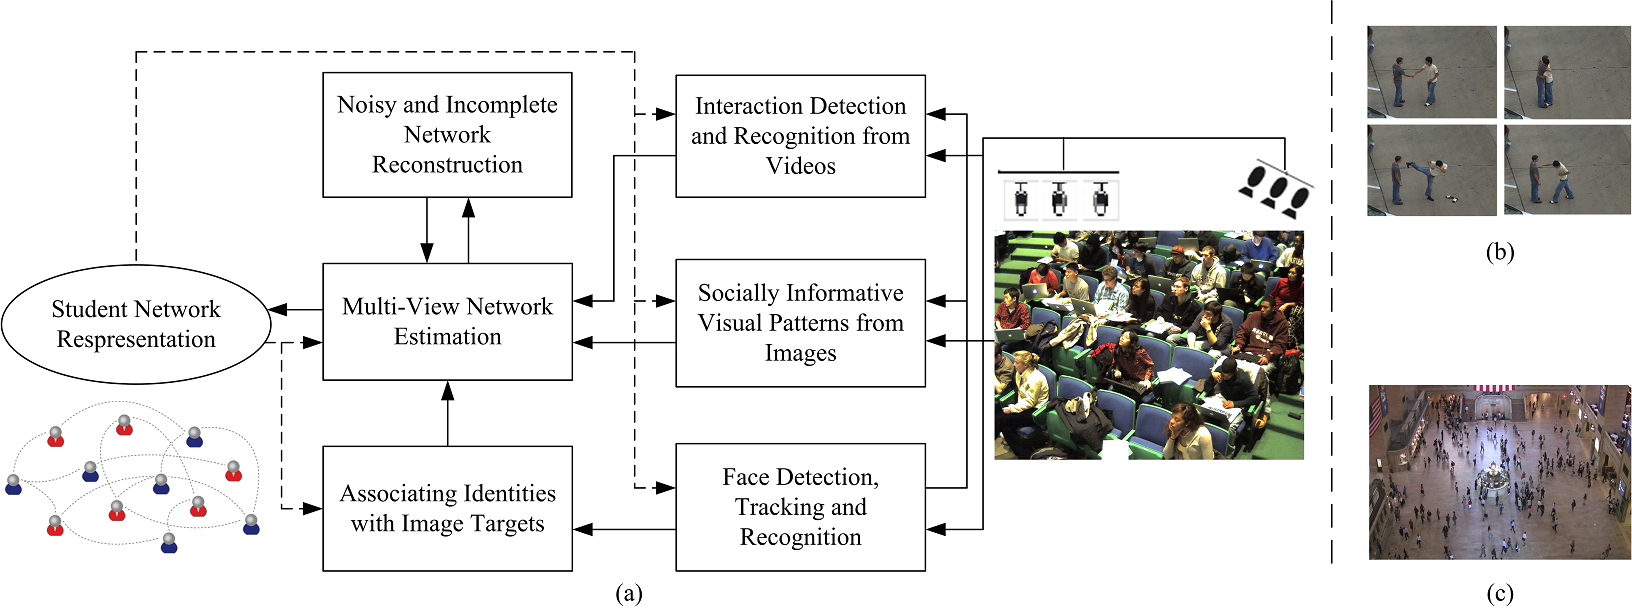
\includegraphics[width=\columnwidth]{prototype_1}
%\end{center}
%\vspace{-0.25in} \caption{\captionsize 
%Interactive classrooms are attractive research testbeds because unlike most existing datasets (b: \cite{UTdata}) they contain diverse behaviors in a real, cluttered environments, and therefore provide strong proxies for social visual analysis in the wild (c: \cite{WangMG09}). We will evaluate our research systems on videos collected from a classroom observation system (a) that already exists at Harvard University.}\label{fig:prototype}\end{figure}



%Our goal is to build a foundation for social analysis in diverse, unconstrained environments like Fig.~\ref{fig:prototype}(c). This is becoming well within reach due to increasing availability of networked camera arrays and advances in practical multi-view detection and tracking (e.g.,~\cite{EshelM10}). These unconstrained environments are fundamentally different from scenarios considered in most existing benchmark datasets for interaction analysis (Fig.~\ref{fig:prototype}(b)), where the interactions involve a pre-determined number of participants; take place in the absence of by-standers or social clutter; and/or are localized  \emph{a priori} in time~\cite{UTdata,Choi:context,Choi:recogtrack,CRIM13}. Because of these  differences, evaluations on existing benchmarks fail to provide meaningful proxies for fundamental progress in widespread social visual analysis.

An encouraging trend over the last several years has been the increasing use of benchmark datasets for evaluating progress on particular tasks. Standardized datasets, such as the Middlebury Stereo Evaluation project~\cite{ScharsteinS02} and the PASCAL VOC Challenges~\cite{Everingham10} have served as catalysts for progress on difficult problems because they create concrete targets that inspire new ideas and allow researchers to evaluate their systems by quantitatively demonstrating improvement. 

As part of the proposed activity, we will build analogous benchmarks and challenge problems for interaction analysis and visual social network analysis in diverse, unconstrained environments. These benchmarks will serve as good proxies for real-world applications like analyzing online photo collections that can be pre-processed with face and body detectors, and analyzing videos from networked camera arrays and surveillance networks (e.g.,~\cite{CamNetRoy}) that can be pre-processed by (multi-view) detection and tracking systems (e.g.,~\cite{EshelM10,CamNetSclaroff}). These scenarios are fundamentally different from those considered in existing datasets for interaction analysis~\cite{UTdata,Choi:recogtrack,Patron-PerezMRZ12}, where the interactions are only weakly socially-relevant; involve a pre-determined number of participants; occur in the absence of non-participating by-standers; and/or are localized \emph{a priori} in space and time. We will create fundamentally different benchmarks and challenge problems that move beyond these limitations and provide better proxies for progress on real-world problems. In addition to enabling our own progress, these benchmarks will be shared to engage our colleagues in our research agenda. 

We will create at least four datasets, two based on images and two based on videos.


%As part of the proposed activity, we will create new datasets and challenge problems that make it possible to measure meaningful progress on social visual analysis, and at the same time, serve as mechanisms to engage the broader research community. To ensure our benchmarks provide effective measures of progress, they will be annotated with ground-truth information about identities, interaction categories, and social relationships. We will create and use two distinct types of datasets. The first type will be based on video collections that are already being collected in interactive classrooms at Harvard University. These datasets will be large (more than 350 camera-hours so far) and will enable evaluation of all aspects of the proposed research program. Because of privacy restrictions they will not be made directly available to non-collaborating research groups, so we will create a second set of  datasets for this purpose.

%As part of the proposed activity, we will create new datasets that make it possible to measure meaningful progress on social visual analysis, and at the same time, serve as mechanisms to engage the broader research community, by enabling the evaluation of certain aspects of the proposed research program (e.g., detecting and recognizing proxemes). These will be presented as ``challenge problems" for the broader computer vision research community. 


\boldstart{Image-based benchmarks}. We will harvest one of our image-based benchmark from personal photo albums embedded in a real social network, such as Facebook, using techniques established by PI Zickler~\cite{Stone2008,Stone2010,PintoZickler2011}. This image corpus will be annotated with body poses, identities, and metadata about the social relationships of co-occurring individuals, thereby enabling the quantitative evaluation of methods for learning and detecting static proxemes, like those in Fig.~\ref{fig:prodic}(b), as well as methods for inferring social relationships and networks. Some aspects of this data, such as the anonymized per-image coordinates of facial and body key-point locations, will be made publicly available to other researchers through the PIs' websites, while sensitive identity and social relationship information will be maintained securely at Harvard University and made available to researchers through secure collaboration mechanisms that are designed in consultation with the Institutional Review Board. PI Zickler has  been successfully using such a secure collaboration process for the classroom videos described below, and it works by having external collaborators: 1) trained in the ethics of research on human subjects through an online course; 2) approved as collaborators by the Institutional Review Board; and 3) conduct their research through remote connections to VPN-protected servers that are maintained by Harvard University.

A second, completely public image-based benchmark dataset will be created by collecting and annotating publicly-available Internet images using keyword searches. These will be made publicly available through the PIs' websites, along with body pose annotations that enable evaluation of learning, detecting, and recognizing static proxemes. We will publish side-by-side comparisons of performance on the private and public datasets whenever algorithms can be evaluated on both. This is a strategy that PI Zickler has previously employed for research on private photo collections~\cite{PintoZickler2011}, and it means that any researcher who evaluates their algorithms on the all-public dataset can quickly obtain estimates of how well those same algorithms might perform in a real social environment.

%In the first image set there will be photos depicting co-occurrences of individuals in various social environments that are collected from internet by keyword search as those in Fig~\ref{flicker}, using which we will learn and detect socially informative proxemes\comment{from pairwise poses and other visual cues, but without estimating social networks}. The second image set will be personal photo albums from Facebook as used in~\cite{Stone2008,Stone2010,PintoZickler2011} where social network information is available, on which we will implement the entire framework introduced .in this proposal. 

%In companion, the first video set will be appropriate seasons and/or episodes of selected TV shows or movies (as shown in Fig.~\ref{fig:socialbehavior}(a)) in which a well-shaped social network exists among characters. Finally, the second video set will be the video collections that are already being collected in interactive classrooms at Harvard University and we will use it as a testbed for reconstructing a specialized social network consisting of class of students. These large-scale datasets will enable evaluation of all aspects of the proposed research program. 


%Because of copyright restrictions, we will make available the annotations for the TV-show/movie dataset but not the original videos, and interested researchers may directly purchase their copies of videos. Because of privacy restrictions, Facebook albums and Harvard Interactive Classroom Dataset may not be made directly available to non-collaborating research groups, and we will create their alternative sets or subsets that public can share. In the following, we provide more introduction to the Harvard Interactive Classroom Dataset that we have been collecting and preliminarily evaluated in \cite{groupdet2013} by the PIs, as well as the Facebook Photo Dataset \cite{Stone2008} by PI Zickler, which serves as a motivating prototype for the new Facebook dataset to be collected.

\boldstart{Video-based benchmarks}. We will create a video-based benchmark dataset, called the \emph{Harvard Interactive Classroom Dataset}, by leveraging video that has been collected by a six-camera array in a large classroom at Harvard University. This system has been developed by PI Zickler over the past few years with funding by the NSF (IIS-0835338, 2009--2012) and the Harvard Initiative for Learning and Teaching (HILT)\footnote{\href{http://hilt.harvard.edu/2012-2013-awards}{http://hilt.harvard.edu/2012-2013-awards}} with the goal of understanding how students learn in interactive classrooms, and a preliminary benchmark dataset derived from it has already been used for computer vision research by the PIs~\cite{groupdet2013}. The observed classroom is ``interactive'' because students frequently engage in the process of \emph{Peer Instruction}, which works as follows. The process begins with a single ConcepTest---a question designed to elicit common student misconceptions~\cite{Crouch:PI,Mazur:PI}---and the students are given a moment to quietly formulate and electronically submit their individual answers. Then they are asked to form ad-hoc discussion groups to try to convince neighboring students of the correctness of their answers. After a few minutes of peer-to-peer discussion, students submit their possibly-revised answers, and this entire activity is followed by the instructor's reinforcement of the main concept. This process is repeated during the time normally devoted to lecture, and education research shows that both high- and low-ability students benefit~\cite{Fagen2002,Hake1998,Okebukola1984,Peterson1979}.

The videos collected by this system present an extraordinary opportunity for developing and evaluating social visual analysis. The observed classroom---crops from which are shown in Fig.~\ref{fig:prodic}(a)---contains a hundred or more individuals engaged in ad-hoc interactions, and this creates a social environment that is fundamentally different from previous video-based benchmark datasets. The utility of this data stems not only from the number and diversity of people it contains, but also from the nature of the interactions, the duration of the observations, and the non-visual sources of metadata available for validation (e.g., audio recordings from 48 microphones; educational outcomes; answers to ConcepTests and exams; gender; age; and ethnicity). The original videos were collected over three months (about 200 camera-hours) and include more than fifty Peer Instruction sessions lasting a few minutes each and involving dozens of small-group discussions.

%Another useful property of the original video dataset comes from the many non-visual sources of metadata that are associated with it. First, for each Peer Instructions session, the dataset contains records of the students' answers to multiple-choice questions before and after their peer-to-peer discussions. Second, thanks to the immense past efforts of collaborating educational experts (funded by other sources and using qualitative analysis techniques like those in~\cite{Scherr2009}), a small number of semantically-meaningful behavioral units have been defined, and occurrences of these behavioral units have been painstakingly annotated in space and time. This means, for example, that when computer vision researchers develop new techniques to discover and detect large numbers of proxemes, they can compare them quantitatively with those identified by human experts. 

As described in~\cite{groupdet2013}, we have already begun developing a suite of computer vision tools for ``pre-processing'' the classroom videos using implementations of face detection and tracking, identity recognition, and head pose estimation that together provide time-varying individual and pairwise descriptors ($\mathbf{f}$ and $\mathbf{g}$ in Sec.~\ref{sec:activity}). These descriptors are affected by many sources of noise---false detections, missed detections, uncertain identities, uncertain pose---and are therefore good proxies for many real-world environments. We will continue developing this pre-processing suite during the award period to extract richer head and body descriptors, such as histograms of flow, space-time interest points, and other features that capture elements of pose, motion, and gestures.

Under supervision by our Institutional Review Board, the classroom videos were recorded with consent from students and instructors and then stored and analyzed on VPN-protected servers. More than 95\% of the observed students provided consent for their videos to appear in academic publications and presentations, allowing disseminate of results through regular academic channels. We will engage external research groups with this dataset in three different ways. First, we will welcome collaborators to analyze the raw data on our VPN-protected servers using the secure protocol described above for images. Second, once we have developed low-level visual descriptors with satisfactory quality, we will anonymize and share these time-varying descriptors as proxies to the original imagery. Third, we will make use of advancing technologies for privacy-preserving social science research---like those currently being developed by colleagues at Harvard University\footnote{\href{http://privacytools.seas.harvard.edu}{http://privacytools.seas.harvard.edu}}---to enable more direct sharing of data.

A second, completely-public, video-based benchmark dataset will be created by annotating identities, and face and body landmarks, in appropriate frames across multiple episodes of a serial television show, such as \emph{The Wire},\footnote{\href{http://www.hbo.com/the-wire}{http://www.hbo.com/the-wire}} that involves an elaborate social network. To adhere to copyright policies, we will publicly share only the annotations for the television show, and not the raw video data. These annotations should be sufficient on their own for benchmarking all of the tasks of Secs.~\ref{sec:activity} and \ref{sec:vis2net}, and they will be time-indexed so that any researcher who desires can purchase their own copy of the raw video and accurately superimpose our annotations.

%In conjunction with our Institutional Review Board, the original classroom videos were recorded with consent from students and instructors, and were stored and analyzed on VPN-protected servers. More than 95\% of students provided consent for their videos to appear in academic publications and presentations, allowing researchers to disseminate their results through regular academic channels. This same consent extends to the subset of the original videos that appear in the Harvard Interactive Classroom Dataset. Researchers from a number of other institutions are already collaborating to analyze this data in a secure manner. Each collaboration happens by the external collaborator(s): 1) being trained in the ethics of research on human subjects through an online course; 2) being approved as collaborators by our Institutional Review Board; and 3) conducting their analysis through remote connections to our VPN-protected servers. These VPN-protected servers are being maintained by the Research Computing Group in the Faculty of Arts and Science at Harvard University, and they will continue to be maintained well beyond the end of the award period.


\comment{
\boldstart{Facebook Photo Dataset}\cite{Stone2008}. The Facebook Photo Dataset was collected from 53 volunteers of active Facebook community members, who agreed to contribute photos and metadata through a web API. Using the API, all photos posted by each volunteer, all photos tagged with any of our volunteers� Facebook friends, all tags associated with any of these photos, and the network of friendships among our volunteers and their friends were archived. A total of 1.28 million tagged photos were retrieved, and all volunteers and tagged friends number 15,752 individuals in all. From this collection, PI Zickler and other collaborators automatically detected and aligned 438,489 face samples that could be associated with the identity labels manually entered by the volunteers. The Facebook dataset was used as the first type of face dataset with social context and enabled the first ``socially-aware" face recognition system \cite{Stone2008}.

In our proposed research, we will retrieve a new photo collection from appropriate online social platforms, and solve the inverse problem: obtaining social network from images. We will inherit the successful data collecting scheme in \cite{Stone2008} by deploying web-based API to volunteers' account, but the new photo collection will be different from the previous dataset in the following aspects. First, we will look into more appropriate online social platforms that emphasize on photo sharing, so that we may obtain more diverse imagery with richer visual cues, e.g.,bodies and scene contexts, than simply faces. Second, we will try to obtain richer annotations about social semantics as well as other metadata than just friendships, with the consent and help from the volunteers. Third, and most important, we will follow a similar strategy as used for the Harvard Interactive Classroom Dataset in producing an publishable version of this dataset, by allowing access to them through our privacy-preserved server, providing anonymized descriptors and metadata, or borrowing other advancing technologies from privacy-preserving social science research.
}


%In conjunction with our Institutional Review Board, we have established a protocol in which classroom videos are recorded with consent from students and instructors, and then stored and analyzed on VPN-protected servers. More than 95\% of students also provide consent for their videos to appear in academic publications and presentations, allowing us to disseminate our research results through regular academic channels. But since the classroom videos cannot be made directly available to research groups other than ours, we will promote reproducible research in three different ways. First, as described in the next section, we will create smaller parallel  datasets that are publicly-available and allow other research groups to evaluate algorithms for certain aspects of social visual analysis. Second, we will welcome interested research groups to collaborate with us to evaluate their algorithms on our classroom data by running their code on our VPN-protected servers. Third, whenever possible we will make use of advancing  technologies for privacy-preserving social science research---like those currently being developed by colleagues at Harvard University\footnote{\href{http://privacytools.seas.harvard.edu}{http://privacytools.seas.harvard.edu}}---to enable more direct sharing of classroom data for research purposes.

%\boldstart{Challenge problems}. An encouraging trend over the last several years has been the increasing use of benchmark datasets for evaluating progress on particular tasks. Standardized datasets, such as the Middlebury Stereo Evaluation project~\cite{ScharsteinS02}, the PASCAL VOC Challenges~\cite{Everingham10}, and the Hollywood database of individual actions~\cite{LaptevMSR08}, have served as catalysts for progress on difficult problems because they create concrete targets that inspire new ideas and allow researchers to evaluate their systems by quantitatively demonstrating improvement. Currently, there are relatively few datasets available for problems related to social visual analysis, and those that do exist consider severely constrained environments that are not good proxies for the real world.

%As part of the proposed activity, we will create new datasets and define challenge problems that engage the computer vision research community in our research agenda. These will be collections of annotated videos that contain interactions staged by informed actors, and they will simulate unconstrained environments by including long videos of large social gatherings. They will be annotated with identities, relationships, and interaction categories, and will thereby  enable the evaluation of certain aspects of the proposed research program (e.g., detecting interaction categories). These will be presented as ``challenge problems" for the broader computer vision research community. We will also publish side-by-side comparisons of our performance on these publicly-shared benchmarks and analogous, but larger, benchmarks derived from our private classroom data. This is a strategy that PI Zickler has previously employed for research on private photo collections~\cite{PintoZickler2011}, and it means that any researcher who evaluates their algorithms on the public datasets can obtain an estimate of how well those same algorithms might perform in a  real classroom environment.

%With this established classroom observation system and these fundamental modules, we have successfully collected and processed a large-scale classroom behavior database consisting of 100 video clips in total. The students are seated in a regular lecture hall and are observed by a camera array with non-overlapping fields of view. The classroom is ``interactive'' because at various times throughout the lecture students are invited to engage in ad-hoc group discussions about problems provided by the instructor. The scale of our database is orders of magnitude larger than state-of-the-art computer vision datasets (e.g. those used in \cite{UTdata,Choi:context,Choi:recogtrack}), in the number of individuals (10-50 students per camera), the number of cameras (6), and the amount of time (100 minutes per camera, per recording, equaling over 3,000 minutes in total). Through a combination of face detection and tracking, we obtained noisy tracks for all students in each monocular video, upon which we developed descriptive modules that directly extract descriptiors such as head pose and body motion, we have also implemented a high-level module for behavior analysis based on similarity between two social groups, as depicted in Fig. \ref{fig:prototype}(b). In this module, the behavior of each individual is represented by a combination of the head pose and the motion of torso and arms (using the method of histogram of optical flows). The social behavior of a group is then represented by the configuration in space and time of the behaviors of its participants. With this social activity representation, the module detects a salient social activity from a new video and retrieves similar social activities from our established database. This functionality is illustrated in Fig. \ref{fig:prototype}(b), where our system has discovered a three-way conversation by identifying the participants of this conversation and the time span (several to tens of seconds) of this event. Based on the behavior representation for this space-time social interaction, the system searches the remainder of the database and retrieves a list of exemplars containing similar social behavior, ranked in the descending order of the similarities with the query. In this way, any manual annotations associated with the query video can be propagated to the top-ranking exemplars, and we are now taking this approach to propagate our manual annotations across the whole database. 








%At the current and initial stage of the effort to bring socialized semantics to computer vision, it can be usually the case that we do not have sufficient social contexts to help improving our target/face recognition, and we are not always specific about what are the meaningful social interactive activities that are most informative for social description. Conversely, we may neither know clearly about what exactly we should distill from images to fulfill a network learning task, nor have concrete knowledge about how the multiple views or overlapping community structures of a network will eventually turn out to be. However, we have argued at the beginning and demonstrated through the four proposed research problems the fact that the two aspects assist and benefit from each other, and an overall socially-aware visual analytical system is our ultimate goal. To this end, our final proposed research will include an attempt for a framework that eventually integrate social information and image understanding and allow them to learn and self-build themselves in an evolving and unsupervised manner.






% !TEX root =  SocialVision2014.tex
\vspace{-8pt}
\section{Broader Impacts}
\label{sec:impacts}
\vspace{-8pt}
A framework that enables social understanding from visual data is critical for computer vision systems to better understand the world from its images. While these topics have received some attention from the research community, it is only now that that we have the data and computational resources to pursue it in any practical, real-world way. The accelerating development of computational infrastructure, the growth of digital video, and progress in detecting and tracking faces and people has finally made this research possible. 

The proposed  program will seize on this opportunity by concentrating our team's resources on the creation of a  framework for social visual analytics.  We will engage many others in its creation: students at carious levels, computer vision researchers, and the broader public. These are critical steps toward a future in which machines can better understand and interact with their environments; and they will usher in radical changes to security, personal robotics, augmented reality, human-computer interfaces, security, and video summarization, to name a few.

Our research will also transform computational research in sociology, economics, and education, by providing access to social patterns that are difficult or impossible to detect with the naked eye. Traditionally, the analysis of interactions has required immense effort by social science experts. Collections of imagery must be viewed repeatedly before salient and meaningful proxemes can be defined, and their occurrences\comment{ in new videos} must be painstakingly and redundantly coded by trained human observers. Our research will transform machine analyses in these disciplines by greatly simplifying the process of defining proxemes, by automating the detection of instances of the proxemes, and by automatically reconstructing social relationships from these detections. This will enable analyses in a much wider set of environments and over transformative periods of time.

Our results will be broadly disseminated in three ways. First, they will be distributed by publications in refereed conferences and journals and by lectures at other institutions.  Second, datasets and source code will be posted online so that they can be easily adopted and extended (see Section \ref{sec:sys} and the Data Management Plan). Third, they will be shared through challenge problem workshops on social visual analytics, held in conjunction with the major vision conferences\comment{ with the small amount of required funding provided by sponsorship agreements}. The research team has an established track record in this type of outreach, with PI Zickler having organized tutorials in vision and  graphics (ICCV 2007, SIGGRAPH 2008) and both PIs having organized workshops on computer vision (CRICV 2009, 2010, CPCV 2011, 2013, VISDA 2013).

\vspace{-8pt}
\section{Curriculum Development Activities}
\label{sec:curriculum}
\vspace{-8pt}
The proposed research program will play an important role in education at both the undergraduate and graduate levels. The fundamental results of this research will be incorporated into the curriculum of a popular computer vision class at Harvard University, \emph{CS283: Computer Vision}, which serves both senior undergraduate students and graduate students at Harvard University. Undergraduates at the junior and senior levels will be also be given opportunities for hands-on research experience in developing components of the proposed framework. This includes extra-curricular and summer research internships that will be funded by future NSF REU supplements, as well as those funded by our institution's many internal funding mechanisms, including the Harvard College Program for Research in Science and Engineering; the Herchel Smith-Harvard Undergraduate Science Research Program; the Harvard College Research Program; and the Mellon Mays Undergraduate Fellowship Program, which is is specifically targeted at underrepresented minorities. Finally, funding will be used to support one full-time PhD student and one part-time PhD student, and these students will be an integral part of both research and educational endeavors in this project. They will participate in all stages, including the design of equipment and algorithms, curricular development, and presentation of results at major conferences.


\vspace{-8pt}
\section{Prior NSF Support}
\vspace{-10pt}
\boldstart{PI Todd Zickler} has been funded through a number of NSF awards to study computer vision, with the most relevant being ``Computer Vision and Online Communities: A Symbiosis'' (HCC-0905243, 2009--2013, \$334,695). \emph{Intellectual Merit}: This award supported research on how to improve face-based identity recognition using a known social network as context~\cite{Stone2010}; how to learn better object and action appearance models from Internet imagery~\cite{owens2011learning,LiZickler2012}; and how to represent social interactions~\cite{groupdet2013} (including the preliminary results in the present proposal). \emph{Broader impacts:} This award contributed to STEM educator development and the creation of a globally-competitive STEM workforce by partially supporting two PhD students and two post-doctoral fellows. It also enhanced infrastructure for research by produced benchmark datasets for face recognition in personal photo collections~\cite{PintoZickler2011} and interaction analysis in a STEM classroom~\cite{groupdet2013}, with the latter also contributing to improvements in STEM education.

\boldstart{PI Ruonan Li} has not previously been supported by the NSF.


\clearpage

\setcounter{page}{1}
\bibliographystyle{plain} \bibliography{NSF_SocialVision,NSF_SocialVision2}


\end{document}

